%%%%%%%%%%%%%%%%%%%%%%%%%%%%%%%%%%%%%%%%%%%%%%%%%%%%%%%%%%%%%%%%%%%%%
%% This is a (brief) model paper using the achemso class
%% The document class accepts keyval options, which should include
%% the target journal and optionally the manuscript type.
%%%%%%%%%%%%%%%%%%%%%%%%%%%%%%%%%%%%%%%%%%%%%%%%%%%%%%%%%%%%%%%%%%%%%
\documentclass[journal=jacsat,manuscript=article]{achemso}

%%%%%%%%%%%%%%%%%%%%%%%%%%%%%%%%%%%%%%%%%%%%%%%%%%%%%%%%%%%%%%%%%%%%%
%% Place any additional packages needed here.  Only include packages
%% which are essential, to avoid problems later. Do NOT use any
%% packages which require e-TeX (for example etoolbox): the e-TeX
%% extensions are not currently available on the ACS conversion
%% servers.
%%%%%%%%%%%%%%%%%%%%%%%%%%%%%%%%%%%%%%%%%%%%%%%%%%%%%%%%%%%%%%%%%%%%%
\usepackage[version=3]{mhchem} % Formula subscripts using \ce{}
\usepackage{color}  % remove this package once you are done
%%%%%%%%%%%%%%%%%%%%%%%%%%%%%%%%%%%%%%%%%%%%%%%%%%%%%%%%%%%%%%%%%%%%%
%% If issues arise when submitting your manuscript, you may want to
%% un-comment the next line.  This provides information on the
%% version of every file you have used.
%%%%%%%%%%%%%%%%%%%%%%%%%%%%%%%%%%%%%%%%%%%%%%%%%%%%%%%%%%%%%%%%%%%%%
%%\listfiles

%%%%%%%%%%%%%%%%%%%%%%%%%%%%%%%%%%%%%%%%%%%%%%%%%%%%%%%%%%%%%%%%%%%%%
%% Place any additional macros here.  Please use \newcommand* where
%% possible, and avoid layout-changing macros (which are not used
%% when typesetting).
%%%%%%%%%%%%%%%%%%%%%%%%%%%%%%%%%%%%%%%%%%%%%%%%%%%%%%%%%%%%%%%%%%%%%
\newcommand*\mycommand[1]{\texttt{\emph{#1}}}
%%%%%%%%%%%%%%%%%%%%%%%%%%%%%%%%%%%%%%%%%%%%%%%%%%%%%%%%%%%%%%%%%%%%%
%% Meta-data block
%% ---------------
%% Each author should be given as a separate \author command.
%%
%% Corresponding authors should have an e-mail given after the author
%% name as an \email command. Phone and fax numbers can be given
%% using \phone and \fax, respectively; this information is optional.
%%
%% The affiliation of authors is given after the authors; each
%% \affiliation command applies to all preceding authors not already
%% assigned an affiliation.
%%t
%% The affiliation takes an option argument for the short name.  This
%% will typically be something like "University of Somewhere".
%%
%% The \altaffiliation macro should be used for new address, etc.
%% On the other hand, \alsoaffiliation is used on a per author basis
%% when authors are associated with multiple institutions.
%%%%%%%%%%%%%%%%%%%%%%%%%%%%%%%%%%%%%%%%%%%%%%%%%%%%%%%%%%%%%%%%%%%%%
\author{Ruchi Lohia}
%\altaffiliation{A shared footnote}
\author{Reza Salari}
%\altaffiliation{Current address: Some other place, Othert\"own,
%Germany}
\author{Grace Brannigan}
\email{grace.brannigan@rutgers.edu(GB)}
\affiliation[Rutgers University]
{Center for Computational and Integrative Biology, Rutgers University, Camden, NJ, USA}
\alsoaffiliation[Rutgers University]
{ Department of Physics, Rutgers University, Camden, NJ, USA}

%%%%%%%%%%%%%%%%%%%%%%%%%%%%%%%%%%%%%%%%%%%%%%%%%%%%%%%%%%%%%%%%%%%%%
%% The document title should be given as usual. Some journals require
%% a running title from the author: this should be supplied as an
%% optional argument to \title.
%%%%%%%%%%%%%%%%%%%%%%%%%%%%%%%%%%%%%%%%%%%%%%%%%%%%%%%%%%%%%%%%%%%%%
\title[An \textsf{achemso} demo]
  {Mechanism underlying conformational effects of the disease-associated Val66Met substitution on the intrinsically disordered region of proBDNF\footnote{A footnote for the title}}

%%%%%%%%%%%%%%%%%%%%%%%%%%%%%%%%%%%%%%%%%%%%%%%%%%%%%%%%%%%%%%%%%%%%%
%% Some journals require a list of abbreviations or keywords to be
%% supplied. These should be set up here, and will be printed after
%% the title and author information, if needed.
%%%%%%%%%%%%%%%%%%%%%%%%%%%%%%%%%%%%%%%%%%%%%%%%%%%%%%%%%%%%%%%%%%%%%
\abbreviations{IR,NMR,UV}
\keywords{American Chemical Society, \LaTeX}
\newcommand{\grace}[1]{\textcolor{blue}{#1}}
\newcommand{\sticky}{proglobular~}
\begin{document}
%%%%%%%%%%%%%%%%%%%%%%%%%%%%%%%%%%%%%%%%%%%%%%%%%%%%%%%%%%%%%%%%%%%%%
%% The manuscript does not need to include \maketitle, which is
%% executed automatically.  The document should begin with an
%% abstract, if appropriate.  If one is given and should not be, the
%% contents will be gobbled.
%%%%%%%%%%%%%%%%%%%%%%%%%%%%%%%%%%%%%%%%%%%%%%%%%%%%%%%%%%%%%%%%%%%%%
\begin{abstract}
Although the role of electrostatic interactions and mutations that change charge states in intrinsically disordered proteins (IDPs) is well-established, many disease-associated mutations in IDPs are charge-neutral. The Val66Met single nucleotide polymorphism (SNP) encodes a hydrophobic-to-hydrophobic mutation at the midpoint of the prodomain of precursor brain-derived neurotrophic factor (BDNF), one of the earliest SNPs to be associated with neuropsychiatric disorders, for which the underlying molecular mechanism is unknown. Here we report on fully-atomistic temperature replica exchange molecular dynamics simulations of the 90 residue prodomain, for both the V66 and M66 sequence.
These g indicate the seemingly subtle substitution may exert its effects by critically adjusting local arrangement of amino acids at the mutation cite, which, in turn, affects the local secondary structure via differential entropic cost of helix formation and global conformational ensemble via differential long-range salt bridging patterns. 
\end{abstract}

%%%%%%%%%%%%%%%%%%%%%%%%%%%%%%%%%%%%%%%%%%%%%%%%%%%%%%%%%%%%%%%%%%%%%
%% Start the main part of the manuscript here.
%%%%%%%%%%%%%%%%%%%%%%%%%%%%%%%%%%%%%%%%%%%%%%%%%%%%%%%%%%%%%%%%%%%%%

\section*{Introduction}

The physiological significance of intrinsically disordered proteins (IDPs), which can explore a wide range of conformational ensembles in their functional form, ~\cite {Uversky2013a,Panchenko2015,Ward2004a,Dyson2005a} is now well-established. More than 33\% of eukaryotic proteins contain disordered regions longer than 30 residues \cite{Ward2004a}, many of which are involved in critical biological functions, including transcriptional regulation and cell signaling \cite{Dunker2005}.  Long intrinsically disordered regions are particularly abundant among cancer and neurodegenerative-associated proteins\cite{Habchi2014,Babu2011}.  

IDP amino-acid sequences tend to be low complexity and include numerous charged residues, often in long repeats ~\cite{Uversky2013a}. In contrast to ordered proteins, in which a complex sequence encodes a well-defined tertiary structure, an IDP sequence determines a heterogeneous conformational ensemble.  More than 35\% of 
IDPs reported in DISPROT ~\cite {Sickmeier2007a} are strong polyampholytes, and their ensemble properties can be predicted using statistical theories of polyampholytes from polymer physics and global properties of the sequence, including the fraction of charged residues and the separation of oppositely charged residues (Fig~\ref{fig1}a)~\cite{Das2015,Das2013a}.  This role is consistent with the long-range nature of electrostatic interactions, which can affect coupling between distant residues in an otherwise disordered structure.  


Although IDP sequences are low-complexity and do not encode a well-defined structure, single residue substitutions can still have functional effects that are significant for the organism.  More than 20\% of disease-associated missense single nucelotide polymorphisms (SNPs) are found in IDPs;\cite{Vacic2012a} although detectable, the relatively subtle functional effects may lead to relatively weak selection pressure, whether positive or negative, allowing the mutation to persist at high frequencies within a population.  Numerous structural and simulation studies ~\cite{Larini2013b,Ganguly2015,Viet2014a,Viet2013,Truong2014a,Zhan2013a,Xu2013a} have demonstrated clear effects of single charged-residue insertion, deletion, or substitutions on conformational ensemble and aggregation of IDPs monomers. Single charged residue mutations or post tranlational modifications that change charges will affect the sequence electrostatics %(such as fraction and separation of charged residues) 
predicted to determine ensemble properties simply from statistical physics models, and in short-chains, can also induce qualitative changes by changing the appropriate regime. ~\cite{Das2015,Larini2013b,Bah2016,He2015}. 
Locally, such mutations can modulate residual secondary structure preferences via forming or breaking local salt-bridges or by introducing helix breaking residues. ~\cite{AlexanderConicella2016,Ganguly2015,Zhan2013a}. Hydrophobicity dependent compaction has been observed in disordered domain of poly(A)-binding protein. ~\cite {Riback2017}.
  
For IDPs with a relatively low fraction of charged residues, typical of the Janus region of the state diagram proposed by Das and Pappu\cite{Das2015,Das2013a} (Fig~\ref{fig1}a), more subtle differences among neutral amino-acids  play an increasingly important role in determining the ensemble.  More than 15\% of disease-associated IDP polymorphisms are substitutions between two charge-neutral residues. ~\cite {Vacic2012a} The extent to which such substitutions in IDPs can affect non-local aspects of the conformational ensemble is uncertain;  such substitution directly affects short-range interactions, and structure-based coupling between distant residues in IDPs is expected to be weak.  Nonetheless, correlations between secondary structure of distant residues has been frequently observed in IDPs ~\cite{Ganguly2015,Iesmantavicius2013}; for example, several cancer mutations in transactivation domain of tumor suppressor p53 can lead to helicity changes in residues sequentially far away from the mutation sites ~\cite{Ganguly2015}.

In structured proteins, contacts between residues distant along the sequence are reflected in the tertiary structure, but developing a framework for describing the analogous property in IDPs has not been straightforward. Among traditional structural biology techniques, NMR has been most useful for characterizing IDPs, but is frequently limited to residual secondary structure (Ref. \cite{Mittag2007,Habchi2014} and references therein). Molecular dynamics (MD) simulations have played a significant role in understanding IDP structure and dynamics ~\cite{Stanley2015,Ithuralde2016,Knott2012b,Invernizzi2013,Abeln2008,Yedvabny2015}, but face limitations on chain length similar to those incurred in simulations of protein folding; most unbiased simulations have been performed in implicit solvent and/or involve chains too short to meaningfully sample contacts between residues far apart on the peptide chain.  Studies of aggregation among multiple shorter monomeric IDPs ~\cite{Levine2015,Pappu2008}  have provided some of the most useful frameworks for considering tertiary contacts between residues which are distantly connected along the peptide backbone.  Point mutations are also known to affect these contacts via differential salt-bridge and hydrogen-bonding formations, with mutations that change charge states affecting conformational ensemble via altered salt-bridge networks. ~\cite{Levine2015} 

Many SNPs in IDPs are associated with neurological, aging-associated neurodegenerative, or psychiatric disorders; despite an exponential increase in the amount of available genetic data, identifying the genetic origins of such disorders has proven remarkably challenging, with few variants identified as replicable predictors of disease.  %despite heritability rates for major disorders reaching 40-70\%.\cite{Alhajji2015} 
One of the earliest identified variants is the Val66Met SNP (rs6265)  in the pro-domain region of Brain-derived Neurotrophic Factor (BDNF), \cite{Notaras2015} a signaling protein %critical for neuronal development and plasticity 
that retains a critical role in neurogenesis and synaptogenesis throughout adulthood(Fig~\ref{fig1}b).\cite{Korte1995} It has been implicated in maintenance of the hippocampus and the mechanism underlying action of numerous antidepressants, \cite{Autry2012,Bjorkholm2016} %(http://www.ncbi.nlm.nih.gov/pmc/articles/PMC3310485/#B15) 
including rapidly acting low-dose ketamine.\cite{Autry2011}  An extensive library of genome-wide association (and even earlier) studies have repeatedly identified the Val66Met SNP as reducing hippocampal volume and episodic memory, as well as predicting increased susceptibility to neuropsychiatric disorders including schizophrenia, bipolar, and unipolar depression, but associations have been inconsistent and population dependent. \cite{soliman2010,Chen2008,Verhagen2010,Notaras2015, Autry2011}. BDNF plays role in orientation selectivity in the visual system ~\cite {Huang1999, Liu2011,Gao2014} and recently, Val66Met has also been associated with reduced visuomotor associative learning and the sensitivity to action observation \cite{Taschereau-Dumouchel2016} 

\begin{figure}[!ht]
 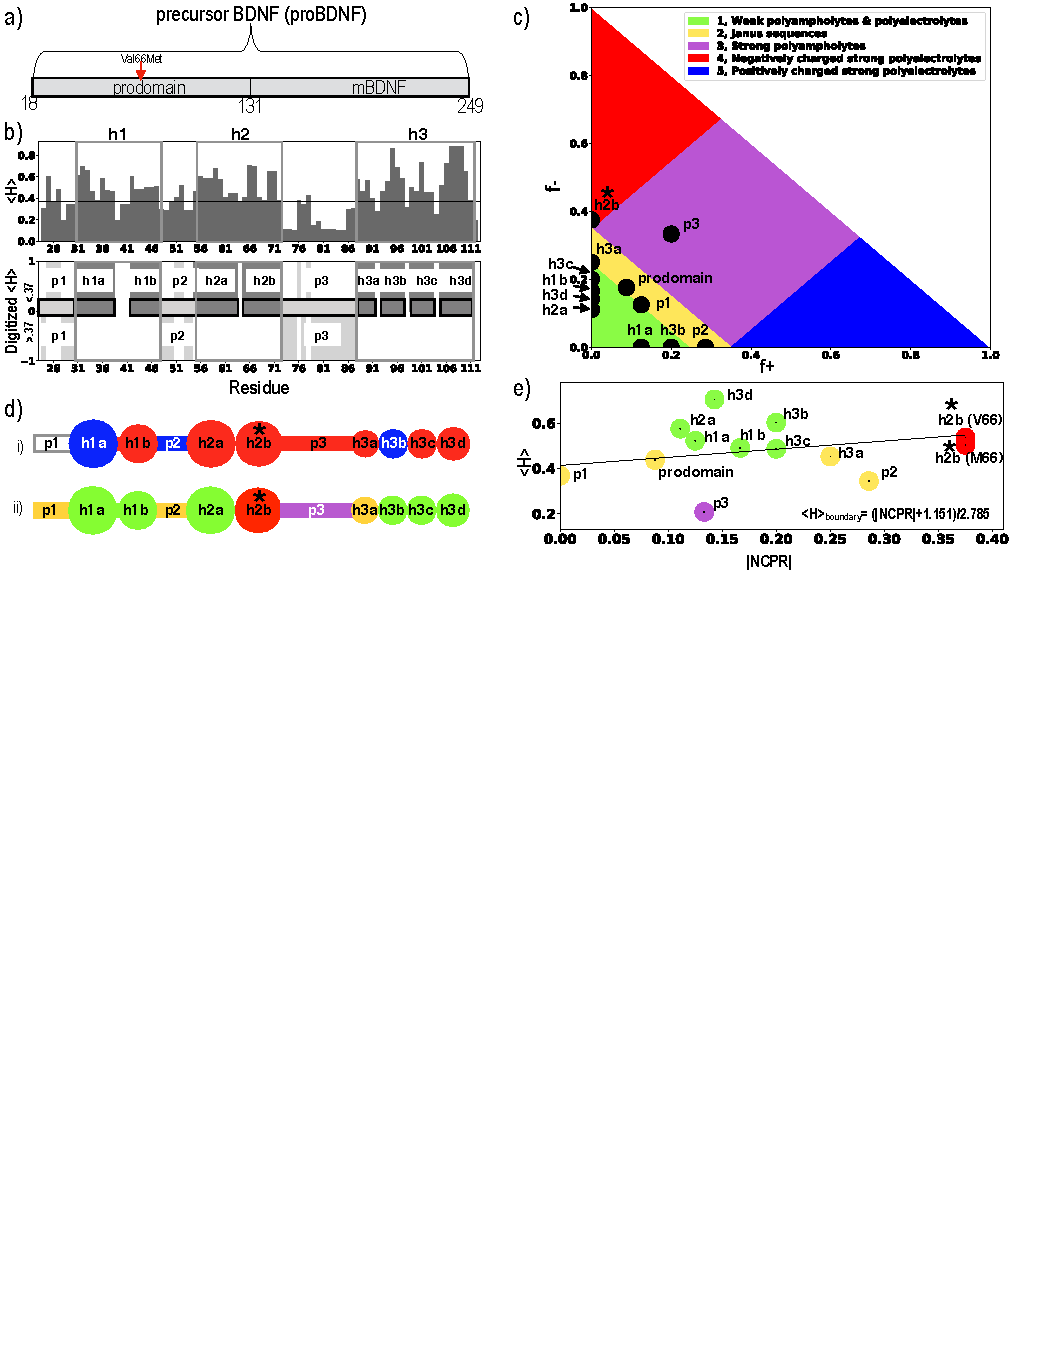
\includegraphics[scale=0.5,width=\textwidth,trim={0 0cm 0 0cm},clip]{../figures/fig1.pdf}
\caption{{\bf Electrostatics in the IDP diagram of states and proBDNF prodomain.} 
a) proBDNF consists of two domains: the prodomain and mature BDNF (mBDNF). b) Diagram of states reported by Ref.~\cite {Das2015,Das2013a}, based on fraction of positively and negatively-charged residues.  As indicated, the V/M66 BDNF prodomain lies on the boundary between the Janus region and the weak polyampholyte/polyelectrolyte regime. 
c) Mean hydrophobicity for the prodomain, based on a sliding window of 3 residues (top) and hydrophobicty based domain identification of prodomain sequence (bottom). The residues are colored according to their charge state. 8 hydrophbic domains (darkgrey) are identified along with 3 domain of low hydrophobicity (dimgrey). d) The cartoon representation of BDNF prodoamin. The domains are colored according to the region found in diagram of states and labelled according to their net charge per residue, showing a highly negatively-charged mid-sequence region (containing the Val66Met SNP)  for V66 (top) and V66\textsuperscript{65+} (bottom). Parts a) is generated with CIDER. ~\cite {Holehouse2017} }
\label{fig1} 
\end{figure}
%/todo increase the label spacing and switch the order for part c).


Difficulties in obtaining unambiguous disease associations at the proBDNF Val66Met SNP using GWAS are paralleled by challenges in characterizing its effects on the properties of the BDNF prodomain using structural techniques.  A crystal structure of a homologous neurotrophic factor in complex with a shared receptor, revealed a well-defined volume corresponding to the prodomain, but which lacked resolvable density.\cite{Feng2010a} 

It was subsequently revealed that the cleaved prodomains ($\sim90$ residues) are found in monomeric states {\it in vivo}, and the M66 (but not V66) form binds to SorCS2 (sortilin-related VPS10p domain containing receptor 2), leading to axonal growth cone retraction.\cite{Anastasia2013} NMR measurements on the prodomain confirmed significant intrinsic disorder for both forms, with differential secondary structure preference around residue 66. ~\cite {Anastasia2013}.  It was not possible to gain any insight into the BDNF prodomain tertiary ``structure'', with uncertainty in interpretation of NMR signal obscuring whether secondary structure is affected far from the SNP, but additional NMR experiments implicated residue 66 in binding of M66 prodomain 
 to SorCS2.~\cite {Anastasia2013}
 
The Val66Met is present in a region with high density of negative charged residues (D61,E64,E68,E69) (Fig~\ref{fig1}c). In this scenario, residue H65 can exist in protonated or neutral charge state in vivo due to it's low pKa. In order to capture the effects of histidine protonation states on Val66Met, we study the Val66 and M66 prodomain in presence of both neutral H65 and protonated H65. For the ease of understanding our observations, the prodomain  sequence is divided into four regions x1: residues 31 to 35, x2: residues 57 to 69, x3:  94-98 and x4: 106 to109 (Fig~\ref{fig1}c).

In this work, we report on unbiased fully-atomistic replica-exchange MD simulations of the 90 residue BDNF prodomain in explicit solvent, for V66,   V66\textsuperscript{65+}, M66 and  M66\textsuperscript{65+} forms.  This sequence falls at the boundary of the Janus and globular domains in the diagram proposed by Das and Pappu. \cite{Das2015,Das2013a} 

\section{New Results and discussion}

%%%%%%%%%%%%%%%%%%%%%%%%%%
%1. Definition of Hydrophobic Domains, including some sequence analysis (kappa, f- f+ of individual domains)  (Figure 1)
%2. Comparison of experimental observables and their computational analogues (Figure 2)
%3. Computational Microscopy (expanded data for computational analogues to experimental results)  : Figure 3 and 4
%4. Discussion of Interdomain interactions (prototertiary structure):
%5. Discussion of Intradomain interactions (including length of secondary structures):
%6. Coupling between inter and intradomain interactions

\subsection{proBDNF sequence decomposition} 

%This subsection should at minimum answer the following questions : 

%-What was the motivation for dividing into domains (i.e. for coarse-graining the sequence)?
%-How do the different domains correspond to the Pappu phase diagram, and which type of domain does the SNP fall in? 
%-How is the SNP domain unique among the proBDNF domains? How is it that we can have a hydrophobic strong polyelectrolyte sequence? 
%-How are the Pappu domains arranged? (i.e. answer: with strong polyelectrolyte at center and globular domains on ends) 
% -What does coarse-graining the sequence reveal about the proBDNF sequence that isn't apparent from just looking at every residue individually? 

\begin{table}[htp]
\caption{Prodomain sequence properties}
\begin{center}
\begin{tabular}{|c|c|c|c|c|c|c|c|c|c|}
\hline
Domains  &  N & NCPR  & Hydropathy  & fcr  & f- & f+ & sigma  & Sequence & Region\\
\hline\hline


-1 & 8 & 0.00 & 3.31 & 0.25 & 0.13 & 0.13 & 0.00 &  EANIRGQG & 2\\
\hline
1a & 8 & 0.13 & 4.70 & 0.13 & 0.00 & 0.13 & 0.13 &  GLAYPGVR & 1\\
\hline
1b & 6 & -0.17 & 4.42 & 0.17 & 0.17 & 0.00 & 0.17 &  TLESVN & 1\\
\hline
1-2 & 7 & 0.29 & 3.10 & 0.29 & 0.00 & 0.29 & 0.29 &  PKAGSR & 2\\
\hline
2a & 9 & -0.11 & 5.18 & 0.11 & 0.11 & 0.00 & 0.11 & GLTSLADTF & 1\\
\hline
2b(V66) & 8 & -0.38 & 4.83 & 0.38 & 0.38 & 0.00 & 0.38 &  HVIEELLD & 4\\
\hline
2b\textsuperscript{65+}	&8	& -0.25&	4.83&	0.50&	0.38	&0.13	&0.13	&H\textsuperscript{65+}VIEELLD	&3\\
\hline
2-3 & 15 & -0.13 & 1.87 & 0.53 & 0.33 & 0.20 & 0.03 & EDQKVRPNEENNKDA & 3\\
\hline
3a & 4 & -0.25 & 4.08 & 0.25 & 0.25 & 0.00 & 0.25 &  DLYT & 2\\
\hline
3b & 5 & 0.20 & 5.42 & 0.20 & 0.00 & 0.20 & 0.20 &  RVMLS & 1\\
\hline
3c & 5 & -0.20 & 4.38 & 0.20 & 0.20 & 0.00 & 0.20 &  QVPLE & 1\\
\hline
3d & 7 & -0.14 & 6.34 & 0.14 & 0.14 & 0.00 & 0.14 &  PLLFLLE & 1\\
\hline\hline
prodomain & 91 & -0.09 & 3.96 & 0.26 & 0.18 & 0.09 & 0.03 & & 2\\
\hline
\end{tabular}
\end{center}
\label{default}
\end{table}%

The BDNF prodomain is 91 residues long (more than 2 times longer than average lengths of IDP's simulated) ~\cite{Henriques, Rauscher2017, Meng2018} because of which looking at the effects of mutation on contacts (\textgreater 91x91) could be cumbersome. To simply things, the prodomain sequence was divided into subdomains based on sequence hydrophobicity. 8 hydrophobic domains and 3 domains with lower hydrophobicity and higher disorder was identified (Fig~\ref{fig1}c). 
The properties of each domain is summarized in the table (Table~\ref{default}).  We characterized each domain on the phase diagram proposed by Pappu et al ~\cite {Mao2010a,Das2013a}. Most hydrophobic domains are weak PA (polyampholytes) with low NCPR (\textless 0.25) and low $\sigma$  (\textgreater 0.2) and are predicted to have globule/compact conformations when isolated ~\cite {Das2013a}. The three identified less hydrophobic domains are comparatively stronger PA (region 2 and 3 on the phase diagram)  with domain 1-2 having high NCPR (\textgreater 0.25) and high sigma (\textgreater 0.2). The two hydrophobic domains, 2b and 3a is a strong electrolyte and boundary region polyampholyte respectively. They have high NCPR and sigma and the two domains are separated with a long (15 residues) strong polyampholyte domain of well mixed charge.

The domain 2b is present at the center and is the only strong polyelectrolyte with highest $\sigma$ and NCPR among all the domains. It has a mix of acidic and hydrophobic residues. Strong polyelectrolytes are predicted to behave as swollen coils, thus the hydrophobic residues in this subdomain would be more accessible to the solvent if present as an independent domain. The Val66met slightly changes the hydrophobicity of domain 2b. However, protonation at residue 65, moves the entire 2b domain from a strong polyelectrolyte region with high sigma to a strong polyampholyte region with low sigma. Since, 2b \textsuperscript{65+} has oppositely charged residues, the hydrophobic residues would be less exposed to solvent. 

The BDNF prodomain by itself is a boundary region polyampholyte with very low NCPR and sigma. 75\% of the IDPs are found to have compositions that place them in either the strong polyampholytic region or the boundary between globules and strong polyampholytes ~\cite {Das2015a}. However, with coarse-graining the BDNF sequence we were able to identify it as an arrangement of 8 hydrophobic domains interconnected with 2 less hydrophobic disorder promoting domains. The Val66met is found in a unique polyelectrolyte domain at the center and is followed by a boundary region domain connected via a strong polyampholyte domain. 


%%%%%%%%%%%%%%%%%%%%%%%%%%%%%%
\subsection{Comparison of experimental observables and their computational analogues}

In order to get accurate structural characterization of proBDNF with MD,  we did  500ns of T-REMD simulations of 30 residue fragment of V66 proBDNF with few popular ff  and water model combinations and proceed with  amber99sb*-ildn-q ~\cite{Lindorff-Larsen2010a, Hornak2006a} with Tip4p-D ~\cite {Piana2015} since it gave best agreement with experimental data obtained by NMR ~\cite{Anastasia2013} (add SI reference).  

\begin{figure}[!ht]
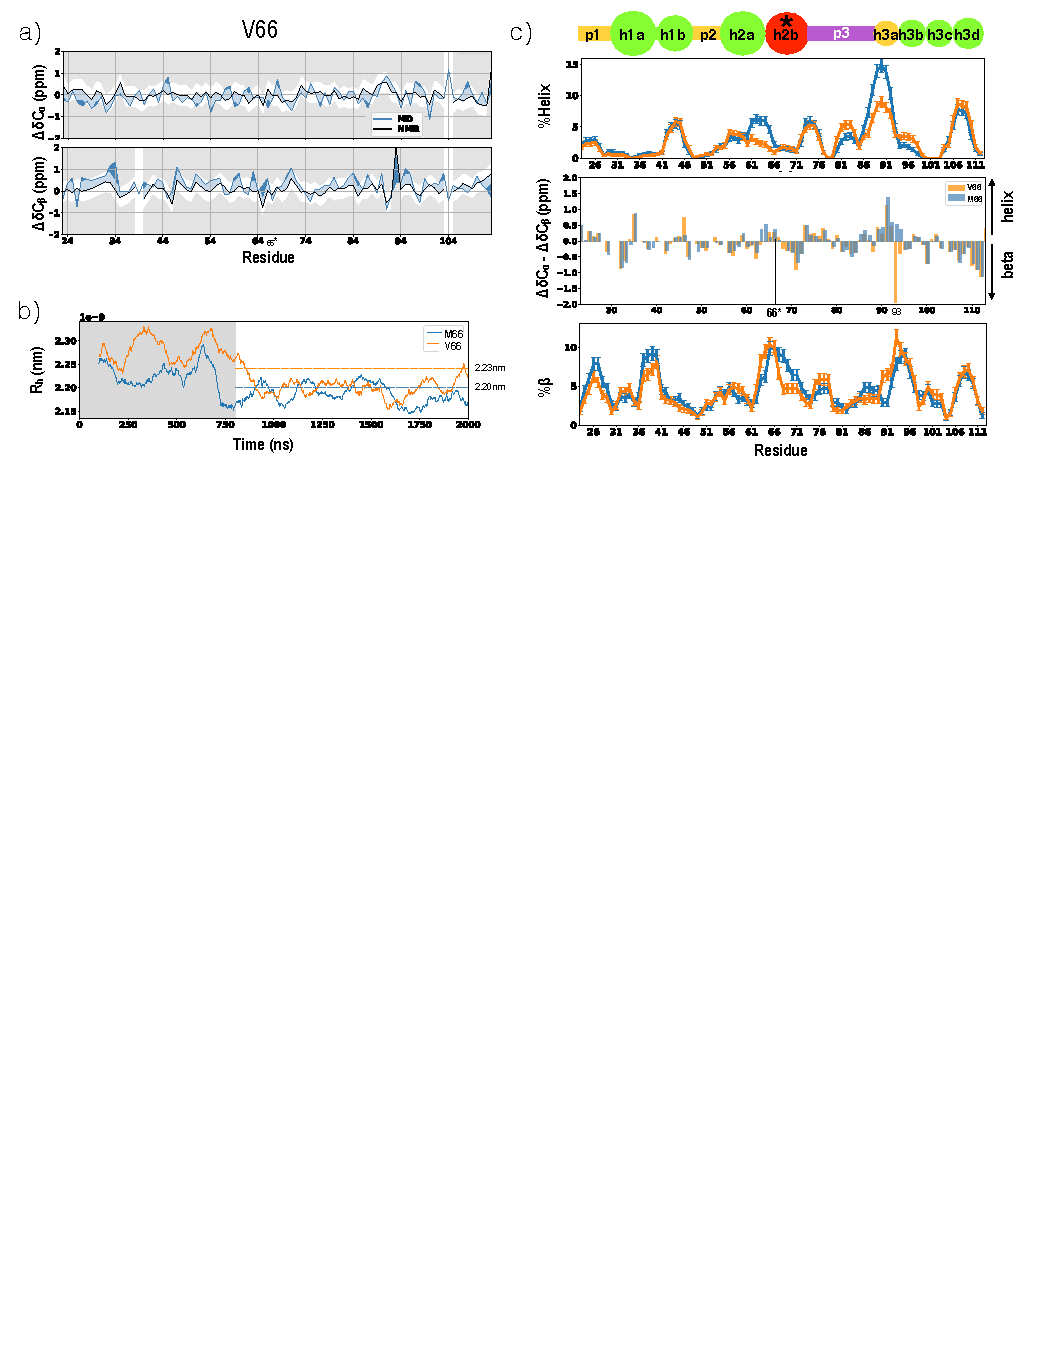
\includegraphics[scale=0.5,width=\textwidth,trim={0 0cm 0 0cm},clip]{../figures/fig2.pdf}
\caption{{\bf Comparison of MD and NMR observables.} a) Comparison of calculated chemical shifts from MD ensembles at 300K and NMR chemical shifts from ~\cite{Anastasia2013}  at 280K,  as described in methods. b) Rh at 100 ns moving  window for V66\textsuperscript{65+} and M66\textsuperscript{65+} vs simulation time. The Rh for V66\textsuperscript{65+} and M66\textsuperscript{65+} converge after 800ns of simulation at 300K. c) STRIDE predicted secondary structure at each residue at 300K (top) and 385K (bottom).  Protonated his65 has increased tendency of forming long helix at residue 66 only for M66. The background of the plots are colored according to residue type: blue-basic, red-acidic, green-polar, white-hydrophobic. d) CA-CB secondary chemical shifts for V66 and M66 from  ~\cite{Anastasia2013}  at 280K. Positive difference indicate helical structure and negative differences indicate beta structure. Region x2 (residues 63-67) and x3 (residues 93-95) have slightly higher tendency of being helical in M66 ( marked with stars ).}
\label{fig2} 
\end{figure}

In order to access the validity of MD generated ensembles, we compare the MD ensembles with experimental data obtained by NMR spectroscopy and NMR diffusion measurements. Fig~\ref{fig2}a compares MD chemical shift and NMR chemical shifts. We get good agreement with NMR chemical shifts; deviations at each residue is \textless 0.5 ppm. Since the chemical shifts for V66 and M66 differ only slightly at few residues positions, we get similar chemical shifts for all 4 simulations as well (very less  \textless 0.5 ppm at each residue) (add SI reference). 
Although there are some localized discrepancies for certain residue types(Y34, Y113, R93, R27), we get discrepancy at same residues for all four simulations. Thus, specific discrepancy is probably reflecting residual force-field inaccuracies. Consistent with intrinsic disorder, helix and $\beta$ propensity for each residue was low for both MD at 300K and NMR data at 280K. It has also been earlier observed that for IDP's with little or no secondary structure,  Amber99sb*-ildn-q with Tip4p-D gives good agreement with experimental NMR measurements. ~\cite {Robustelli2018}.
The simulated hydrodynamic radii calculated using Hydropro ~\cite {Ortega2011} of V66 (2.21 nm) and M66 (2.18 nm) are in excellent agreement with the experimental values (2.24 nm and 2.20 nm respectively) (Fig~\ref{fig2}b). This method has been used earlier to validate IDP ensembles ~\cite {Rauscher2015, Meng2018} and it confirms that the overall dimensions of the protein is reasonable.  This is not surprising as Tip4p-D has been optimized to reproduce the dimensions of disordered proteins ~\cite {Piana2015, Robustelli2018}. 

Most of the IDP simulations studies have been performed on smaller IDP fragments (residues 3-42) ~\cite{Henriques, Rauscher2017, Meng2018} . We performed the explicit solvent replica simulations of 91 residues, which was computationally challenging and thus we carefully accessed the convergence of our simulations. All replicas were able to diffuse in the temperature range 300K to 385K (replica round trip number \textgreater 7) (Fig S1). The Rg for V66 and M66 converge after 800ns of simulation at 300K (Fig~\ref{fig2}b). We discarded the first 800 ns of the trajectories as conformational equilibration. The Rg distribution of all four simulations are unimodal (Fig~\ref{fig4}b). 


NMR studies ~\cite{Anastasia2013}  found increase in helical tendency for M66 at region x2 (residues 64,65,66) and region x3 (residues 90 to 94) ( marked with stars ) and decrease in helical tendency at region x1 (Fig~\ref{fig2}c). To look into the effect of mutation on residual secondary structure, we compare the helix tendency at every residue for each of the four simulation (Fig~\ref{fig4}c). Consistent with NMR experiments, M66 and M66\textsuperscript{65+} has increased tendency of forming $\alpha$-helix at region x1 when compared with V66 and V66\textsuperscript{65+}(Fig~\ref{fig2}c).
%todo for comparing MD and NMR secondary structure I need to do d2D calcualtions

%%%%%%%%%%%%%%%%%%%%


%%%%%%%%%%%%%%%%%%%%

\subsection{Interdomain interactions (prototertiary structure)}

%--------- domain level
%change the cutoff in contact maps
%--Purely based on the domain properties (not individual residue stuff yet), what interdomain interaction preferences would we expect (if any)?
%--What do we actually observe (in the WT, ancestral version)
%--Does it agree with our expectation?
%--How does the V66M hydrophobic mutation change these preferential interactions?  (Not "why" yet, just how)
%--V66M doesn't change any of the domain properties (does it?) - is there still a way for us to interpret  preferential interactions purely on the domain level? (i.e. 3a is Janus sequence which is highly sensitive to small changes in interactions)
%--How does  65+  change  interdomain interactions, and is it consistent with what we'd expect based on how it affects properties of domain 2b?
%--Are changes in interdomain interactions consistent with changes in radius of gyration?
%a metric for the strongest contact formed in each domain

\begin{figure}[!ht]
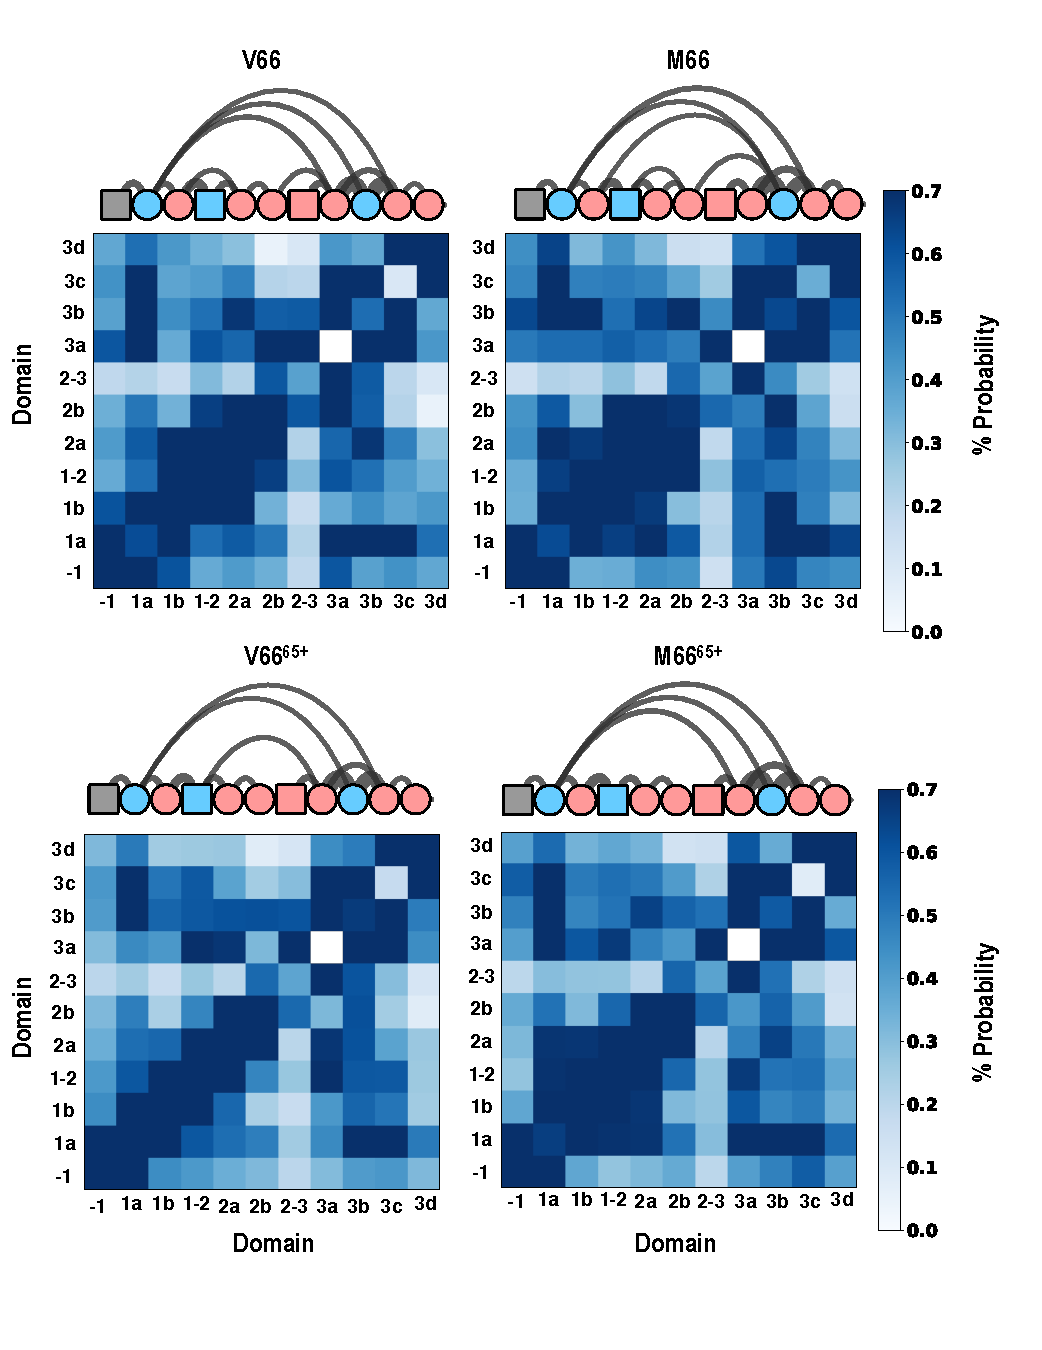
\includegraphics[scale=0.5,width=12cm,trim={0 0cm 0 0cm},clip]{../figures/fig4m.pdf}
\caption{{\bf Contact maps of inter-domain contact .} a) The backbone tertiary-contact network is made for all four simulations.  
 }
\label{fig4m}
\end{figure}

In order to understand the effect of Val66Met on prodomain ensemble, we look at the inter-domain contacts for each form. The normalized probability of inter-domain interactions is shown in (Fig~\ref{fig4m}), measured as described in the Methods. It has been observed that for weak polyampholytes compaction results from decreased FCR with charged residues on the surfaces of globules ~\cite{Das2013a}. Therefore, in general hydrophobic domains with opposite charges will have strong contact preference, with higher sigma having even higher preference. 
Indeed, we observe strongest interaction preference between neighboring domains with opposite charges and high sigma. Domain 3b has strong interactions (\textgreater 2.5\%) with domains 3a and 3c. This brings domain 3a and 3c to be in close contact as well. Domain 3c consistently forms strong contact with oppositely charged hydrophobic domain 1a in all 4 simulations.

The strong hydrophobic polyelectrolyte domain 2b is expected to form strong contacts with other domains due it's exposed hydrophobic residues and high sigma. Indeed, we find strong interactions of domain 2b with 3a and 3b in V66 and M66 respectively (Fig~\ref{fig4m2}). For V66, strong contact is formed at 3a:1a and between same charged domains 2b:3a. This is surprising that the negatively charged domain 2b forms strong contact with negatively charged 3a domain. 3a also forms contact with 1a, however, 3a and 1a are oppositely charged. M66 looses the contact 3a:2b and 3a:1a and forms stronger contact at 3a:3b. Additionally, M66 also has stronger interactions at 3b, i.e. 3b:2b and 3b:1b, 3b:-1, 3b:3d. 

Among all the contact differences formed between V66 and M66, only contact 2b and 3a is formed between domains with same (negative) NCPR. Val66Met only reduces the hydrophobicity at domains 2b slightly, then how can it change the interactions with domain 3a ? Domain 3a is a boundary region polyampholyte and their conformation is very sensitive to it's environment including secondary structure preferences ~\cite{Das2013a}. It is possible that Val66Met changes the secondary structure preference between residue 66 (2b) and 3a.

textbf{Among all the residue level interactions at domain 2b:3b in M66, M66 and M95 form strong contacts. Give the reference that earlier also these references are known to play a significant role. } %todo add the figure showing 2b:3b interaction in M66

\begin{figure}[!ht]
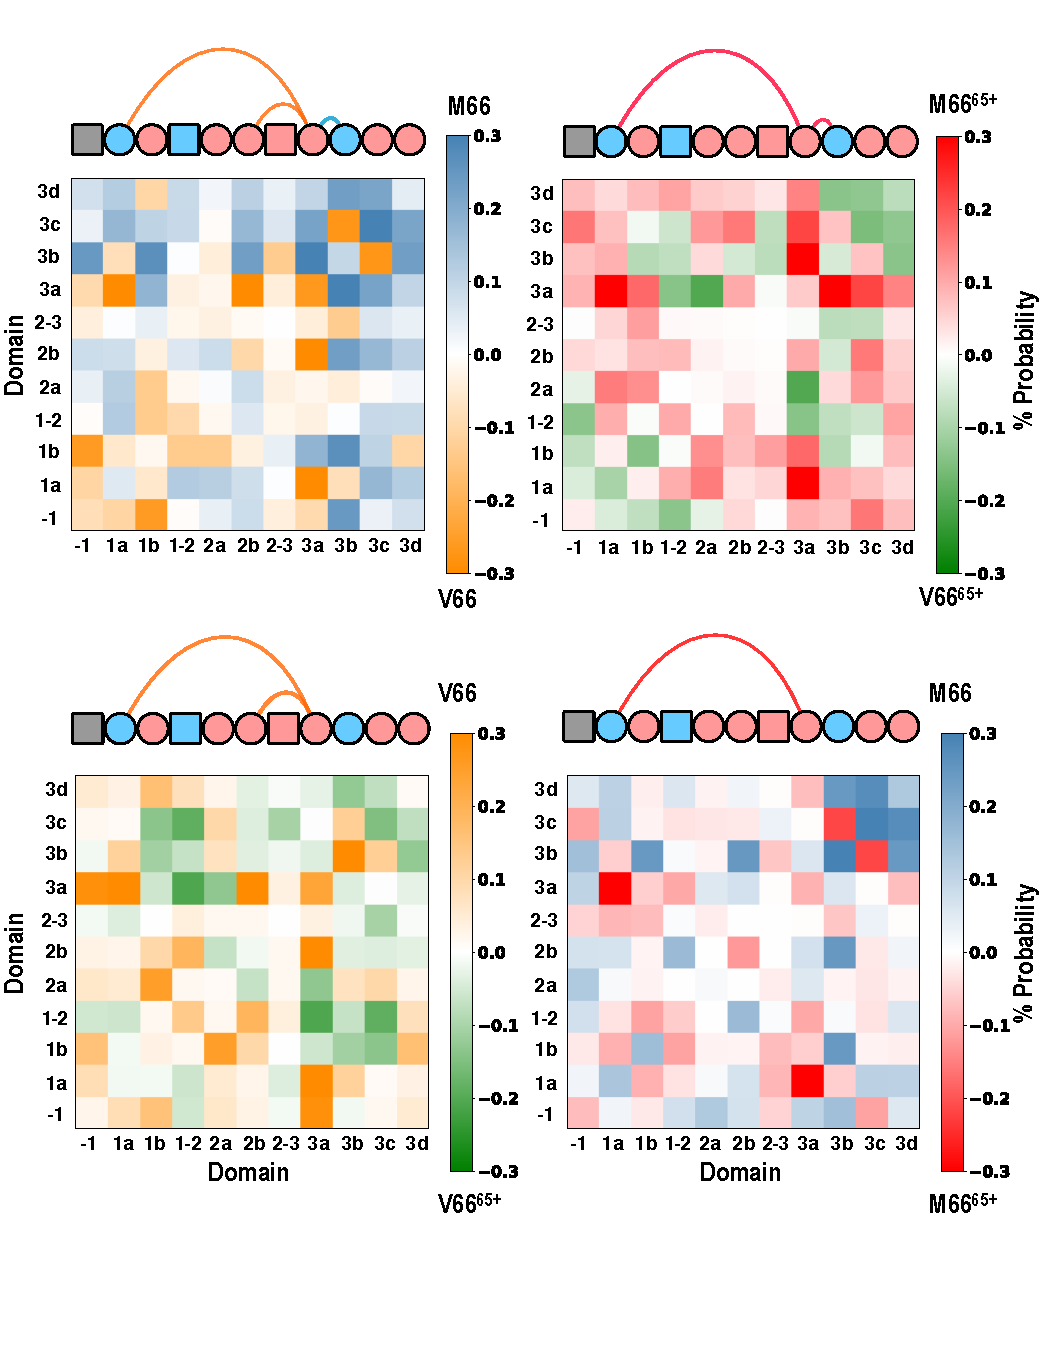
\includegraphics[scale=0.5,width=12cm,trim={0 0cm 0 0cm},clip]{../figures/fig4m2.pdf}
\caption{{\bf Difference contact maps of inter-domain contact .} a) The backbone tertiary-contact network is made for all four simulations.}
\label{fig4m2}
\end{figure}

These contact maps for the entire ensemble indicate far more tertiary contacts between domain 2b and adjacent domains for V66 and M66 when compared with the protonated H65 (Fig~\ref{fig4m2}).  It has been earlier observed that fraction and distribution of charged residues along the disordered protein sequence determines it's contacts. Domain 2b which was a negatively charged polyelectrolyte, expected to behave as swollen coil independently now changes to strong polyampholyte with reduced sigma due to H65\textsuperscript{+} and is expected to form coil ~\cite{Das2013a}. In-fact, we observe more interactions of 2b with itself in M66, as expected for a domain which has a mix of both positive and negative charges.

For V66 protonation looses strong inter-domain contacts formed earlier at 2b:3a and 3a:1a and gains weak contacts at 1-2:3a and 1-2:3c. This is not surprising, since 1-2 (no longer 2b) and 3a are oppositely charged domains with high sigma. 
For M66 protonation weakens the contacts at 2b:3b, 3b:1b but maintains strong contact at 3a:3b and gains strong contact at domain 3a:1a. 

M66\textsuperscript{65+} gains strong contact at 3a:3b and 3a:1a when compared with V66\textsuperscript{65+}, whereas V66\textsuperscript{65+} forms it's most persistent contact at 3a:2a.  We find that boundary region domain 3a is very sensitive to both mutation and protonation and can form strong contacts with domains with same NCPR.
We also find that M66 consistently forms strong contact at 3a:3b and 2b forms stronger contacts with rest of domains when compared with V66. This could explain, the slightly more compact states of M66 and M66\textsuperscript{65+}  when compared with V66 and V66\textsuperscript{65+}.  For both V66 and M66, protonation at 65 reduces inter-domain contacts at 2b, thus we find slight increase in Rg in H\textsuperscript{65+} when compared with their respective neutral H65 forms. In the later section we would find out that why we get stronger contact preference for domain 2b in M66 when compared to 2b in V66.
%\todo chen showed that domain 3a, 3b are essential for the protein to function.
	

%%%%%%%%%%%%%%%%%%%%%%%%%%%%%%%%%%%%INTRADOMAIN%%%%%%%%%%%%%%%%%%%%%%%%%%%%%%
\subsection{ Intradomain interactions (protosecondary structure)}
%I think you should be pretty comfortable with this section, but you should to restrict them to 2b and 3a, and consider them separately
Next we look at the effect of mutation and protonation on protein intradomain contacts and eventually the secondary structure.  The alpha-helix propensity indicates that both mutation and protonation effects the helix propensity at several residues. To carefully differentiate the helix propensities we compare the length of simultaneous helix formed at each residue (described in methods) for each form. Among all the intra-domain contacts, domain 2 (2a:2b) has the strongest change (\textless 90\% stronger than other intra-domain contacts) followed by domain 3 (3a:3b).

\begin{figure}[!ht]
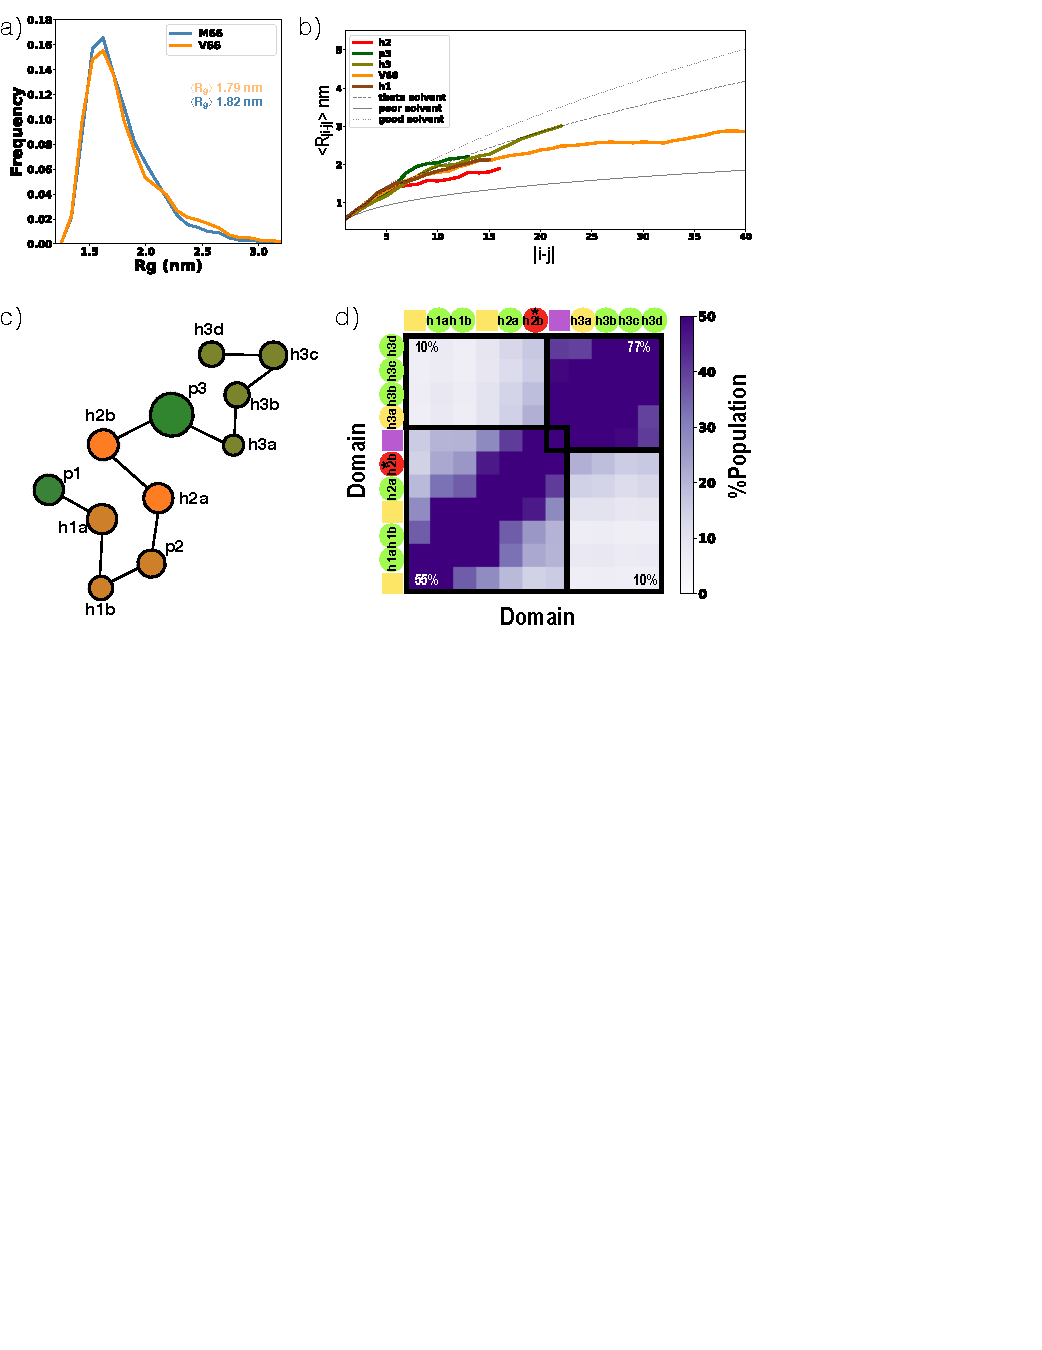
\includegraphics[scale=0.5,width=12cm,trim={0 0cm 0 0cm},clip]{../figures/fig3.pdf}

\caption{{\bf Simulation predicted secondary structure properties.}
a) Difference in helix length (top) and beta length (bottom) for each residue. In agreement with the experiment, we find higher tendency of forming longer helix at regions x2 and x3. V66 has higher tendency of forming beta at region x3.  b) Helix length distribution at each residue when 66 is in the helix region of ramachandran map (methods) }

\label{fig3} 
\end{figure}

\subsubsection{2a:2b}
%QUESTIONS: 
%In what way does the residual secondary structure in the vicinity of the mutation/protonation site change? 
%In what way does the length of secondary structure elements change? 
%What could explain these differences (without -yet- invoking interactions with other domains)?
%END QUESTIONS
Val66Met mutation in both protonated and neutral H65 states, consistently increases the frequency of long helix ( \textgreater 6 residues) formed at region 2 (both 2a and 2b) (Fig~\ref{fig3}a). 
Reduced entropic cost of helix formation in M66 when compared with V66 possibly contributes to the increased helix formation. Creamer et. al. ranked the entropic cost of helix formation for apolar side chains using simulations of a (Ala)\textsubscript{8} sequence with the 'guest' amino acid at the center and reported higher entropic cost helix formation for Valine when compared with Methionine \cite{Creamer1992}. 
For both V66 and M66, protonation slightly increases the helix propensity at most domains, except at domain 2a in M66\textsuperscript{65+}. 
When protonated at 65 in M66, the helix propensity shifts from helix at residues 59-67 (9 residues) to  even longer helix at residues 62 - 71 (10 residues).

Among all intra-domain contacts, all four simulations has stretch of strong contacts formed at i:i+3. Two hydrophobic residues commonly form strong contacts (\textgreater 60\%) among all residue pairs. A60:F63 forms strong contact for all four simulations. 

M66 has strong preference for residue F63:M66, F63:I67 whereas V66 has strong preference for I67:L70. M66\textsuperscript{65+} consistently has stronger preference at F63:I67 when compared with V66\textsuperscript{65+}.  A previous study from Faure et al ~\cite {Faure2008} analyzed the frequency of two amino acids contact within 1230 protein chains from Protein DataBank (PDB) and found that Methionine (M) has also a strong affinity with Phenylalanine (F) and itself.

When protonated, V66 looses contacts at L59:H65 and gains contacts at H65:E68, V66:F63. When protonated, M66 looses contacts at G55:A60 and gains contacts at H65,V66 and I67. Protonation gains contacts, this is not surprising, as protonation at H65 decreases electrostatic repulsions in the otherwise negatively charged polyelectrolyte domain. It has been earlier observed that  the intrinsic disorder and acidic residues keep two hydrophobic motifs from driving collapse. Instead, the most-active variants keep their aromatic residues exposed to the solvent. ~\cite {Staller2018}.

%b) Helix stabilization in M66 by preferential contact formed between M66:F63. We looked at the weight of the contact formed at every residue pair separated with two residues (Fig~\ref{fig5}). Either two hydrophobic residues (L43:V46, A60:F63,A87:Y90 ) or  two residues with opposite charge (E73:K76), commonly form strong contacts (\textgreater 65\%) for both V66 and M66.
 
%Among others 
\subsubsection{3a:3b}
%QUESTIONS:
%In what way does the residual secondary structure or length of secondary structure elements change for each mutation and protonation state? (i.e. what should the reader be noticing)
%It was placed in the Janus sequence region based on f+ and f-, so are the changes in secondary structure associated with differences in interactions between charged residues? 
%END QUESTIONS
Val66Met mutation in both protonated and neutral H65 states, consistently increases the frequency of long helix ( \textgreater 6 residues) formed at region 3(both 3a and 3b) (Fig~\ref{fig3}a). 
For both V66 and M66, protonation slightly increases the helix propensity at domain 3a. 
When protonated at 65 in M66, the helix propensity further increases at residues 95 and 98 (3b).

\begin{figure}[!ht]
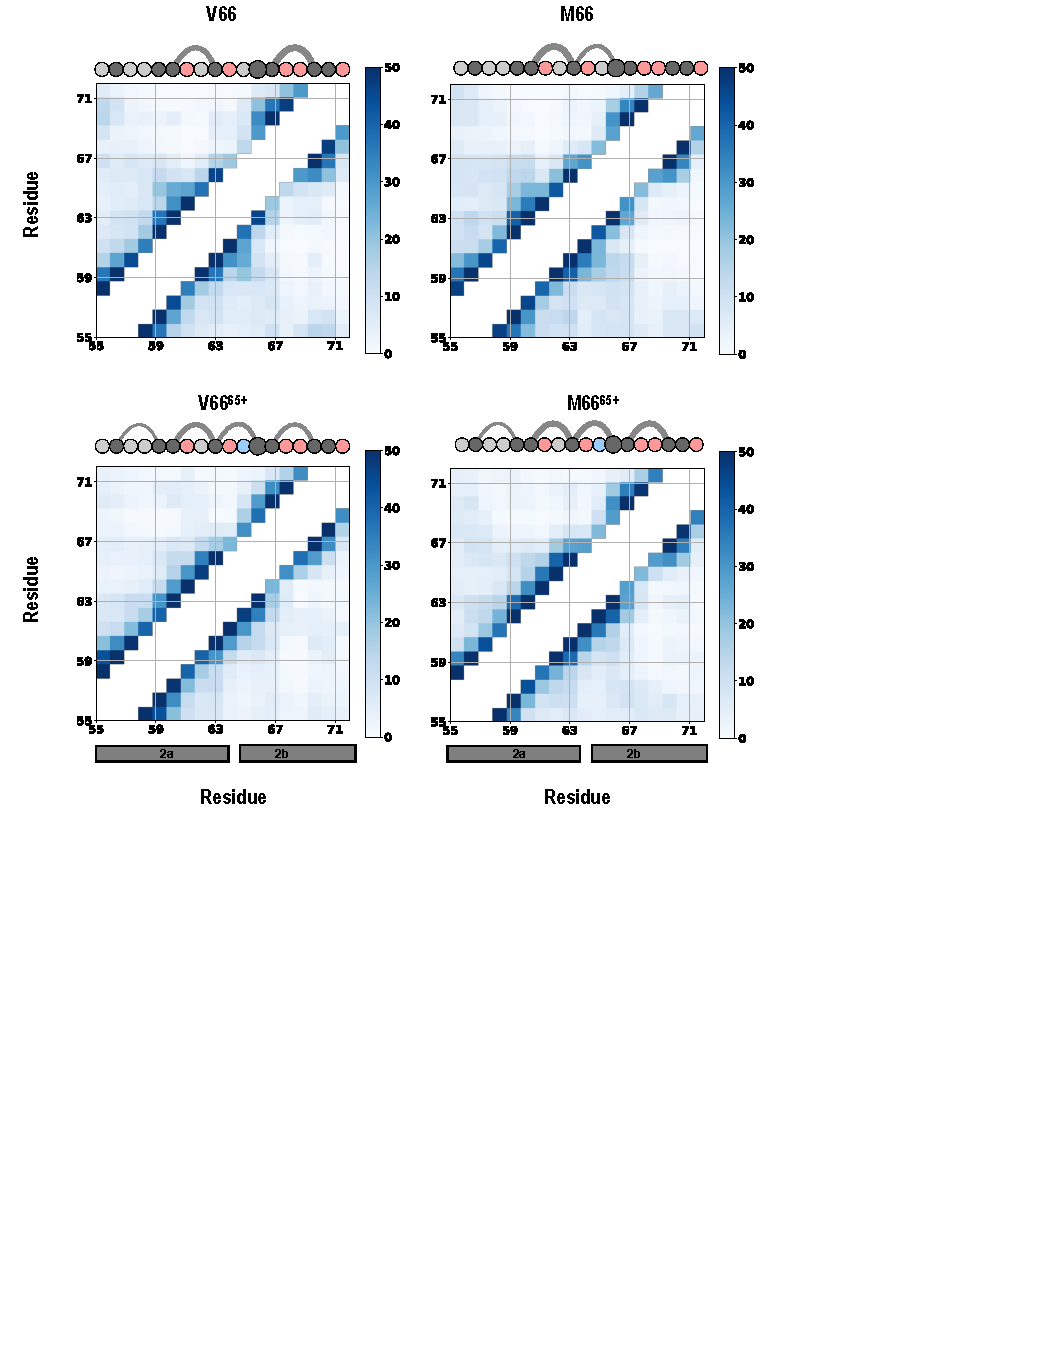
\includegraphics[scale=0.5,width=12cm,trim={0 0cm 0 0cm},clip]{../figures/fig-3-1.pdf}

\caption{{\bf Intra-domain contacts at domain 2.}
Weight of contact formed at every residue pair. M66 forms strong contact at residue M66:F63, whereas V66 forms strong contact at residue I67:L70.}
\label{fig5} 
\end{figure}

\begin{figure}[!ht]
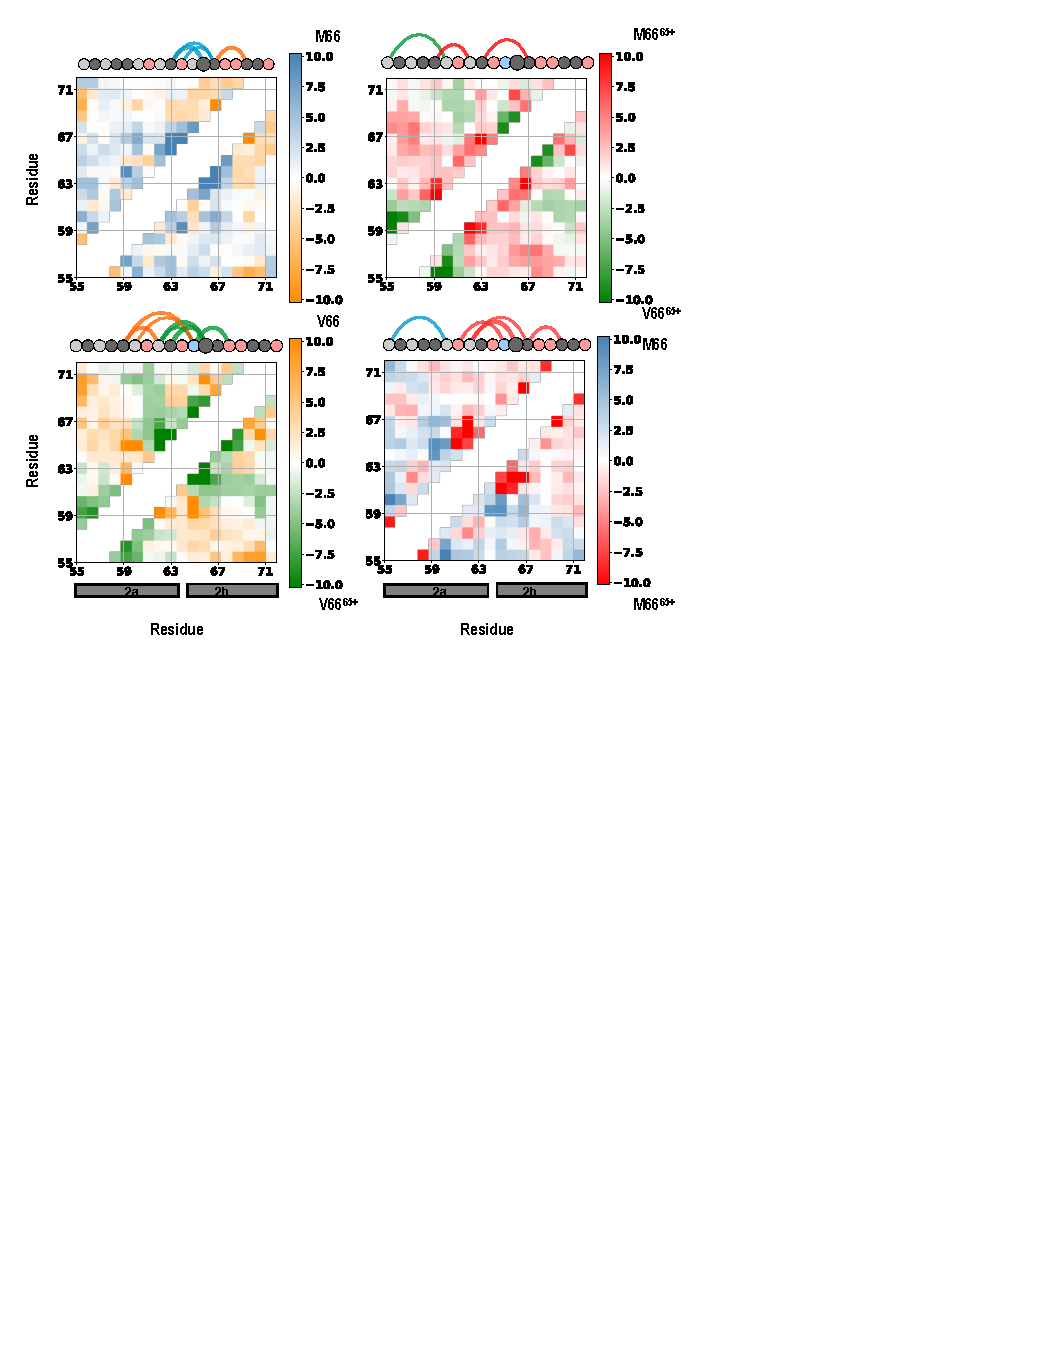
\includegraphics[scale=0.2,width=12cm,trim={0 0cm 0 0cm},clip]{../figures/fig-3-2.pdf}

\caption{{\bf Difference in Intra-domain contacts at domain 2.}
M66 forms strong contact at residue M66:F63, whereas V66 forms strong contact at residue I67:L70.}
\label{fig5} 
\end{figure}

\begin{figure}[!ht]
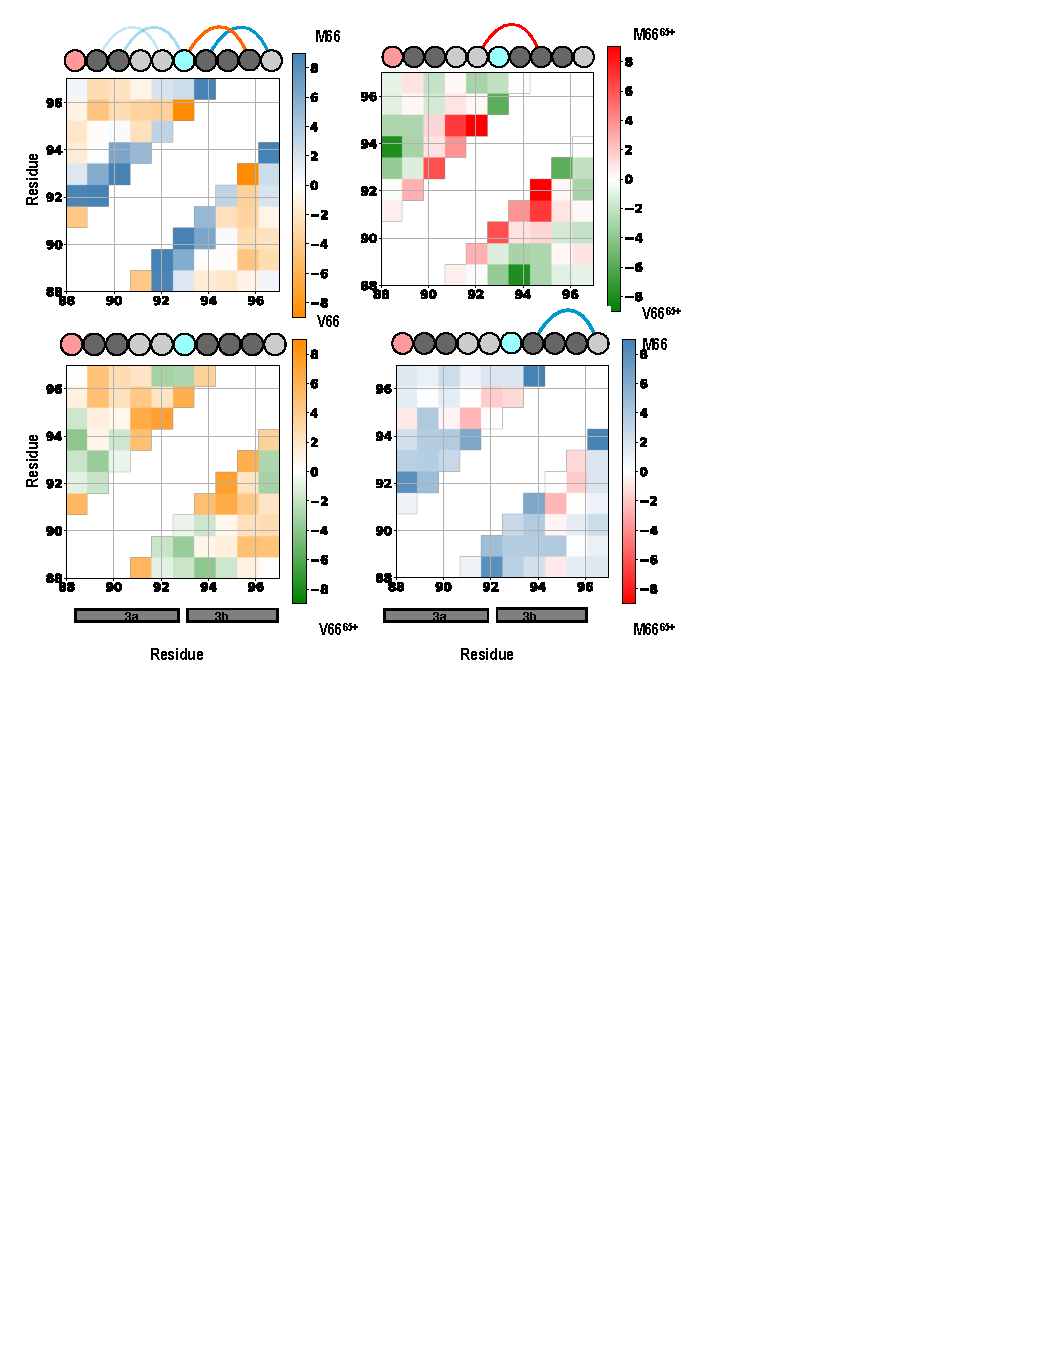
\includegraphics[scale=0.5,width=12cm,trim={0 0cm 0 0cm},clip]{../figures/3a_3b.pdf}
\caption{{\bf Difference in Intra-domain contacts at domain 2.}
 }
\label{fig6}
\end{figure}

\clearpage
\subsection{Secondary structure (intra-domain) and tertiary structure (inter-domain) coupling} 
\textbf{Long helix at 2a:2b are formed along with interactions at domain 2b:3b in M66}\\
Inter-domain contacts: Helix at 2a:2b forms strong contact at domain 2b:3b.\\
Inter-domain contacts (residue level): M66:M95 is formed. This supports helix at residue 66.\\
Helix coupling: Long helix at 2a:2b (8 residues) is coupled with small helix at domain 3a (5 residues). Long helix at domain 3a is coupled with short helix at domain 2a. \\
Intra-domain contacts: domain 2a:2b, F63:M66 and domain 3a:3b, Y90:R93\\
\textbf{Long helix at 2a:2b are formed along with interactions at domain 2b:3b in M66 protonated form}\\
Inter-domain contacts: Consistent with M66,  M66\textsuperscript{65+} helix at 2a:2b forms strong contact at domain 2b:3b.\\
Inter-domain contacts (residue level): M66:M95 is formed. This supports helix at residue 66. Additionally, stronger contact is formed at residue L70:R93. \\
Helix coupling: Long helix at 2a:2b (9 or more residues) is coupled with long helix at domain 3a (8 or more residues).\\
Intra-domain contacts: domain 2a:2b, F63:M66, M66:L70 and domain 3a:3b, Y90:R93. \\
The helix at M66\textsuperscript{65+} shifts from 8 residue helix at 59-66 to 9 residues helix at 63-71. This has several implications.\\
Longer helix is formed at domain 2b and 3a. This happen due simultaneous contact formations at residues M66:L70:R93.

Like any other protein, inter-domain contacts, intra-domain contacts and secondary structure are coupled in prodomain. In M66 forms (both protonated and non-protonated at 65), the contact formation at 2b:3b occurs simultaneously with helix formation at 2b or 3b. 
We observe that the contacts formed at  2b:3b is stabilized with Met66:Met95 interactions. This is not surprising, it has been earlier observed that Met:Met, Met:Phe interactions are stronger than aromatic:aromatic ~\cite {Gomez-Tamayo2016}. 
Probably the gain of interactions at 2b:3b looses 2b:3a interactions in M66 when compared to V66.


\begin{figure}[!ht]
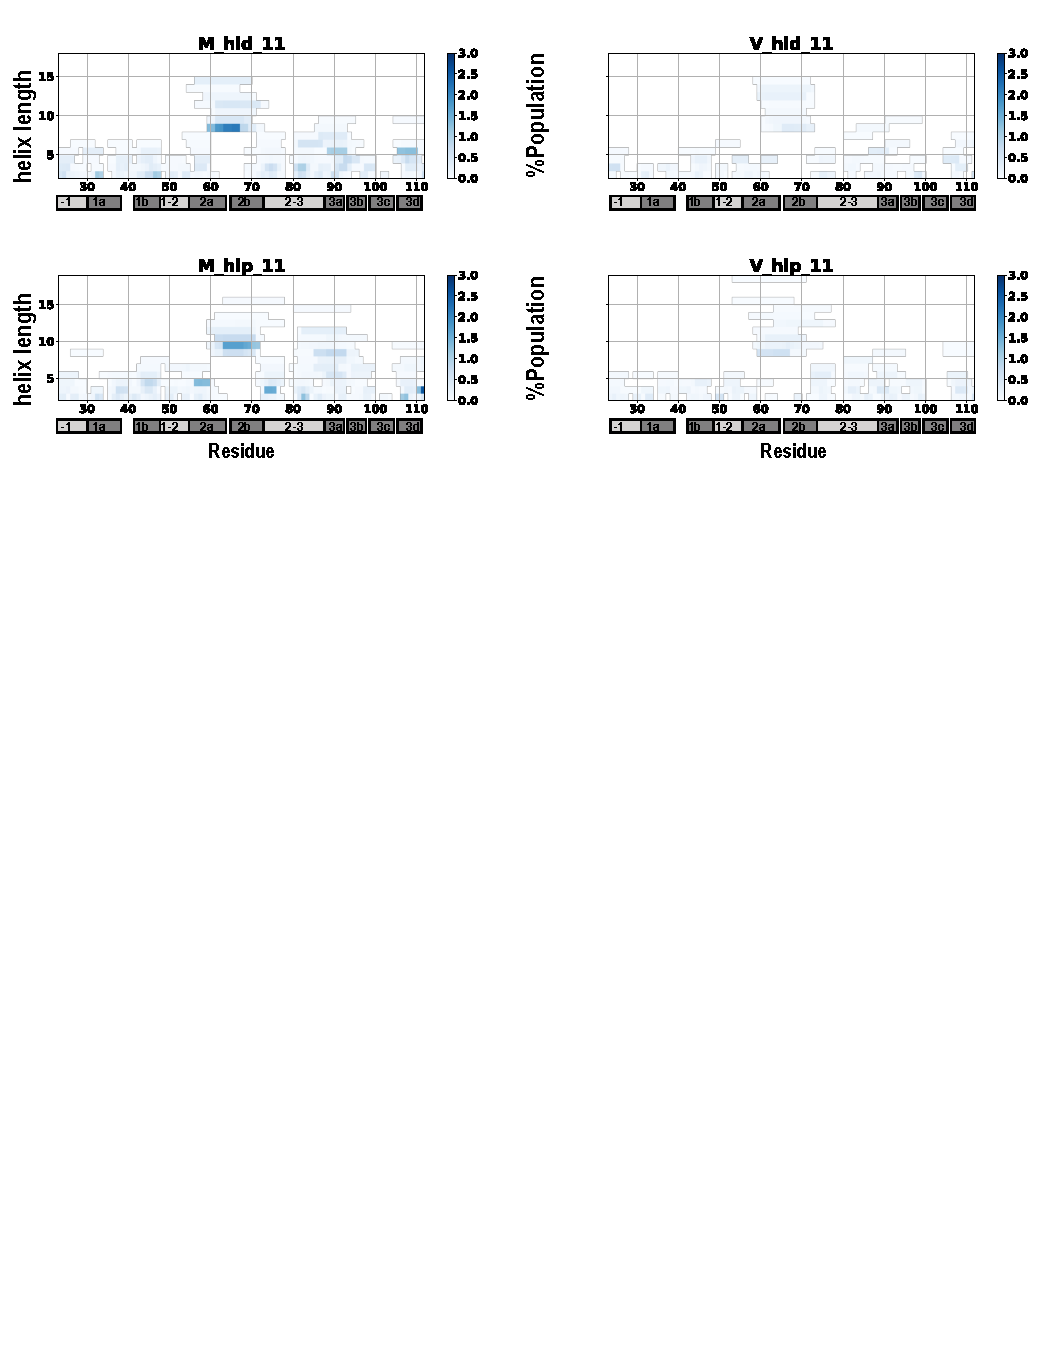
\includegraphics[scale=0.5,width=12cm,trim={0 0cm 0 0cm},clip]{../figures/n1.pdf}
\caption{{\bf Helix coupling at domain 2a:2b and 3a.}
 }
\label{fig6}
\end{figure}

\begin{figure}[!ht]
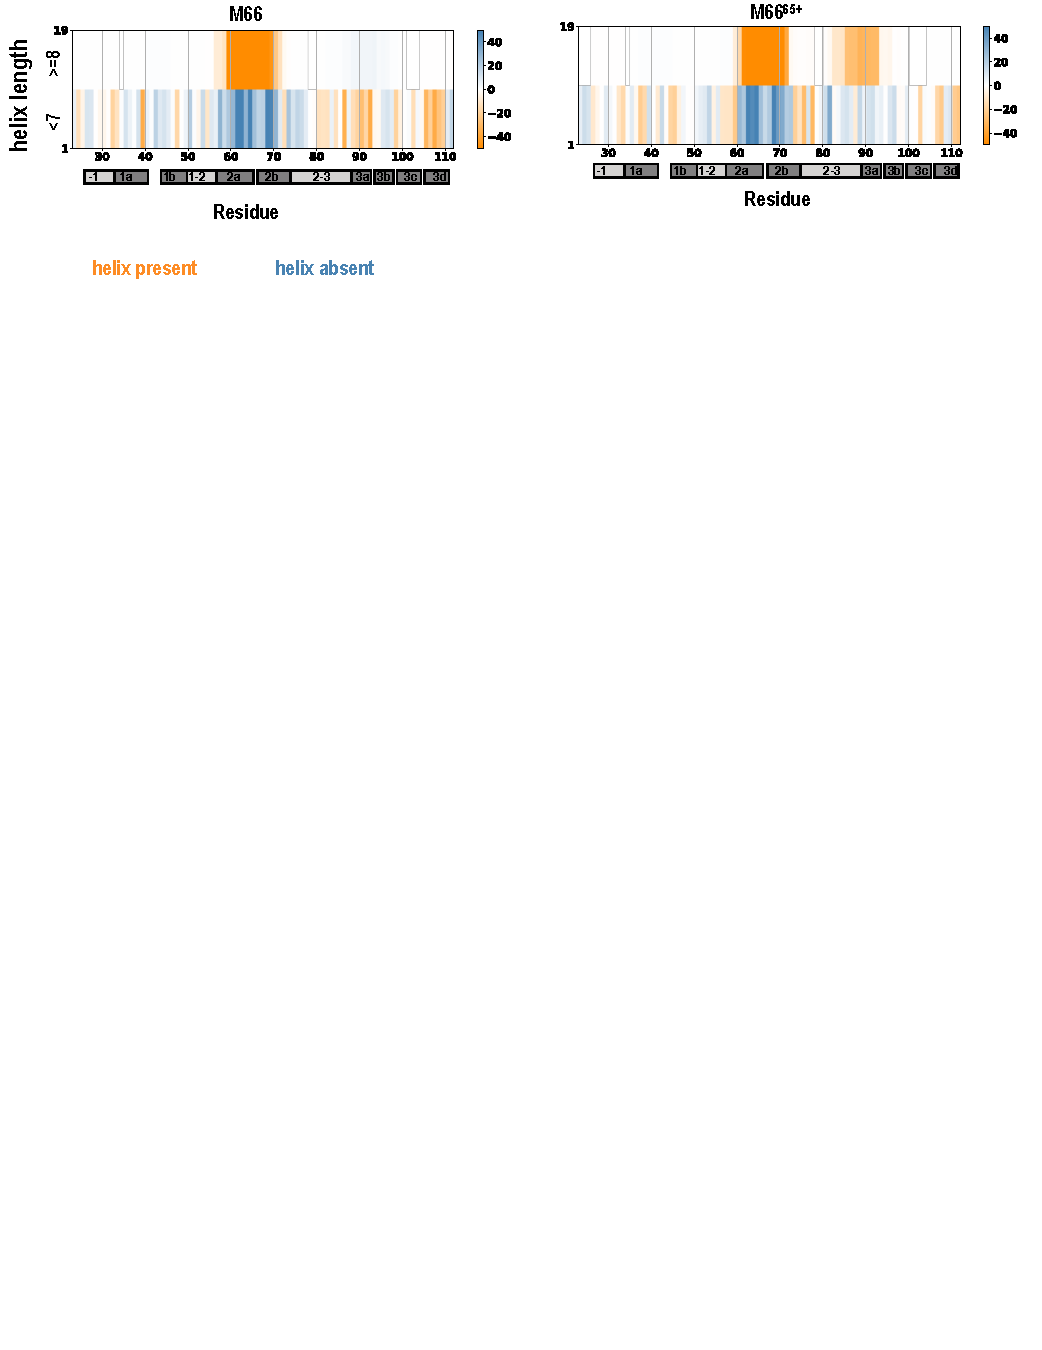
\includegraphics[scale=0.5,width=12cm,trim={0 0cm 0 0cm},clip]{../figures/n2.pdf}
\caption{{\bf  Helix coupling at domain 2a:2b and 3a.}
 }
\label{fig6}
\end{figure}

\textbf{In V66 when 2b:3b are in contact, there is formation of beta structures}\\
Inter-domain contacts (residue level): V66:S92 is formed. This supports beta structure at residue 66.\\
Intra-domain contacts: In V66, I67:L70 is present in domain 2b.\\
In the above results we found that V66 intradomain interaction is unique; it has the weaker intradomain contact at 63:66 and stronger intradomain contact at 67:70.  V66 also has the weakest probability of helix formation at 66. In quantative terms, V66 has 50\% higher probability of contacts when 63:66 is absent and 67:70 is present simultaneously when compared with other three simulations (40\% vs 20\%).\\
%probability is directly proportional to sample size
2b:3a forms strong contact in V66 when compared to any other simulations. 50\% of the contacts formed at 2b:3a is formed simultaneously with the absence of 63:66 and formation of 67:70. At domain 3a:3b, the contact 90:93 breaks when 2a:3b is formed in V66.\\

\textbf{3a is janus sequence so beta pairing trend can be removed by very slight environmental changes.}
In agreement with the Janus region placement of domain 3a, we observe strong secondary structure formation of both helix and beta tendency at domain 3a. In V66 3a forms beta pairing with various domains including domain 2b whereas in M66 domain 3a forms helix pairing with domain 3b. The strong interaction at domain 2b:3b, supports helix formation at 3a:3b. 

 
%
%We also look at the temperature dependence of helical structure in prodomain. At 385K, the helix at residue 66 increases (\textgreater 2\%) for all V66, M66, V66\textsuperscript{65+}, but M66\textsuperscript{65+} has strongest preference (\textgreater 5\%) (Fig~\ref{fig4}c). Thus,  increased hydrophobic interaction with temperature (F63:M66) along with reduced electrostatic repulsion (H65:E69) in M66\textsuperscript{65+} favors helix formation.

%\subsubsection{Effect of changing charge state on contacts within domain 2 }
	
%%%%%%%%%%%%%%%%%%%%%%%%%%%


\subsection{Coupling between inter and intra-domain interactions} 
%%%%Questions
% 1) In V66, there is a much stronger contact between 2b and 3a than in any of the other systems.  Are there ways in which the 2b or 3a intradomain interactions are also different for V66 from any of the other systems? [Provide 1-3 ways] 
% 2) For each difference, does the difference/correlation extend to fluctuations within the V66 sequence? (for example, one way might be that 3a is also much less likely to form helix in V66 than the other sequences. Considering just the V66 simulation, for frames when 2b-3a contact is formed, are 3a helices shorter/less probable than frames when no 2b-3a contact is formed?) 





%%%ON HOLD for now%---------residue level
%--Do the specific residues participating in interactions change for V66M, *particularly* *between within 2b and 3a*
%--(optional) Do the specific residues participating in interactions change for 65+, *particularly* *between within 2b and 3a* (edited) 
%focus on contacts between far residues
%update the cytoscape maps with 1 contacts
%update the cytoscape map
%I will have to look at the contact which are formed together between domains
%	\textbf{M66 supports helix formation at residue 93}



%In V66, 
%2b:3a - 66-91, 72-91
%3a:1a - 33:90

%In M66
%3a:3b - 89-93 - contact 66-95
%2b:3b - 66-95 - contact 63-66

%In M66ip
%2b:3b - 70-93 - helix at 95
%3a:1a - 34-89 - long helix at 66

%In v66ip
%1-2:3a -  54-91 - forms 65-68 salt-bridge

%We next examined the increased helix tendency at residue 93 from Val66Met substitution. We find structures forming helix at 93 are in contact with residue 66 in at-least 25\% of it's population in M66\textsuperscript{65+} (Fig~\ref{fig6}). The gain of this residue specific interaction in M66, probably increases helix formation at 93 when compared with V66. 



\begin{figure}[!ht]
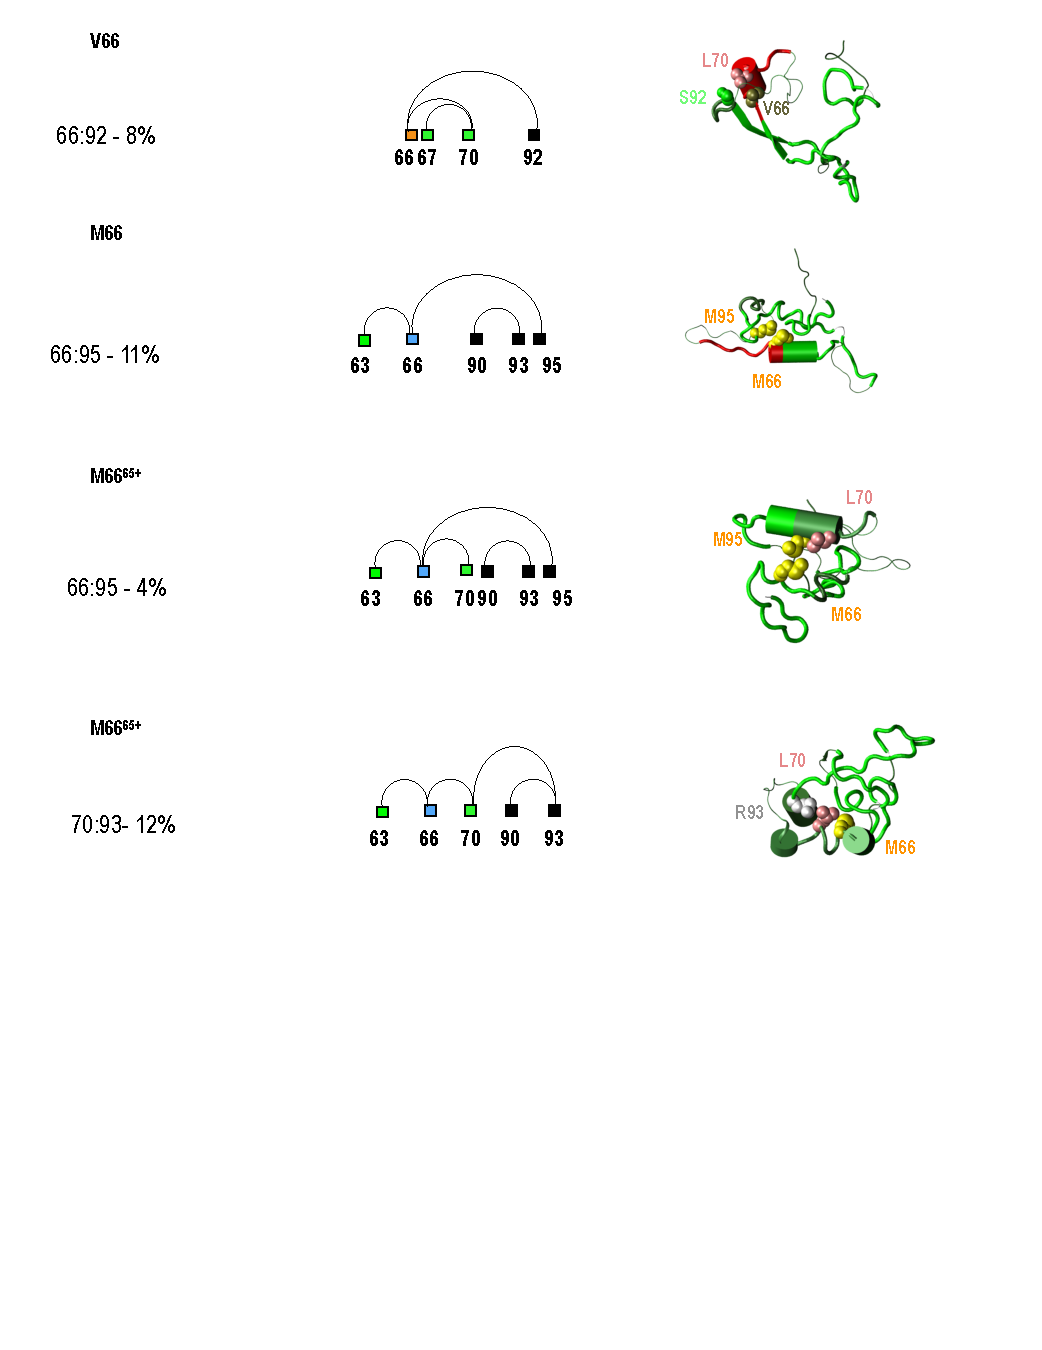
\includegraphics[scale=0.5,width=12cm,trim={0 0cm 0 0cm},clip]{../figures/n3.pdf}
\caption{{\bf Secondary structure and long range contacts coupling in prodomain.}
 }
\label{fig6}
\end{figure}



%We next examined the increased helix tendency at residue 93 from Val66Met substitution. We find structures forming helix at 93 are in contact with residue 66 in at-least 25\% of it's population in M66\textsuperscript{65+} (Fig~\ref{fig6}). The gain of this residue specific interaction in M66, probably increases helix formation at 93 when compared with V66. 
	
\newpage


\section*{Conclusion}

We have carried out ~.5ms of fully-atomistic MD simulation of the 90 residue prodomain of brain-derived neurotrophic factor with protonated and neutral His65 state, for both with and without the disease-associated Val66Met mutation.  

Anastasia et al~\cite{Anastasia2013} observed differential kinetics for interactions between BDNF prodomain and SorCS2; M66 binds more strongly at residues H65 to L71 with SorCS2, whereas V66 binds more strongly at residue Y90 to V94. 
The stronger binding at residue M66 could be attributed to either a) ability of M66 to form alpha-helix at residue 66 when compared with V66 or b) stronger hydrophobic contact at residue M66 with the SorCS2 hydrophobic residues or combination of both a) and b). 

Residue 66 possess several meaningful properties, beyond including the disease-associated mutation of our original interest. It is a) neutral residues inserted in a stretch of acidic residues constituting the most highly charged region of the protein and b) directly adjacent to the sequence midpoint at E68.  We have not yet isolated which of these contribute to the critical role of residue 66 in forming strong tertiary interactions, and it is possible that overlap of (a) with (b) is intrinsic to the protein design.  

	
%\subsubsection{Finer resolution: Effect of Val66Met on *which* residues are doing the interaction}

%The V66M mutation affects which contacts within the domains form the long-range contacts, particular between x1-x2 and x2-x3. 
%		
%Several specific contacts are shown that are found in a significant number of frames for either V66 or M66, but not in the other one.   
%We observe few long-range contacts with significant differences in V66 and M66 with p  \textless  0.0001. \grace {The cross-over N is \~15 frames ?} .  We find that the differences we observe in long-range contacts are strongly correlated with contacts at residue 66,67 (i) and (i-3).
%
%Conventional contact maps provided little useful insight into tertiary structure for either forms of the protein, which was consistent with the intrinsic disorder and frequent transient interactions among neutral side-chains. Identification of contact residues yielded several persistent, weak long-range interactions at 300K for both sequences, which can be represented along a single axis (Fig~\ref{fig4}). 
%

\begin{figure}[!ht]
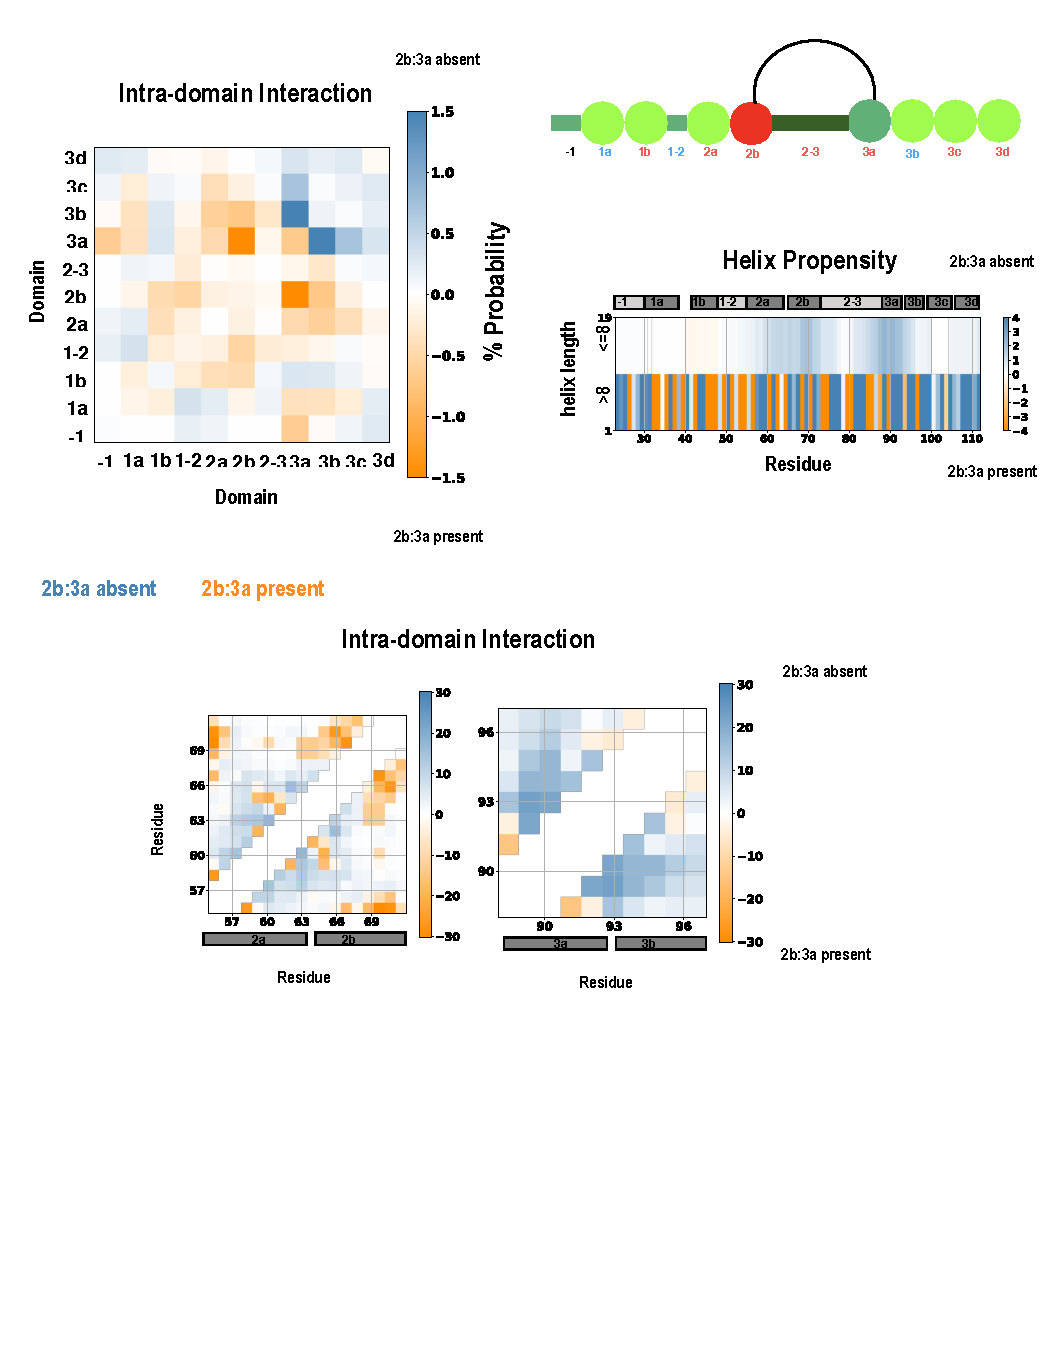
\includegraphics[scale=0.5,width=12cm,trim={0 0cm 0 0cm},clip]{../figures/coupling_2.pdf}
\caption{{\bf 2b:3a contact formation in V66.}
 }
\label{fig6}
\end{figure}

\begin{figure}[!ht]
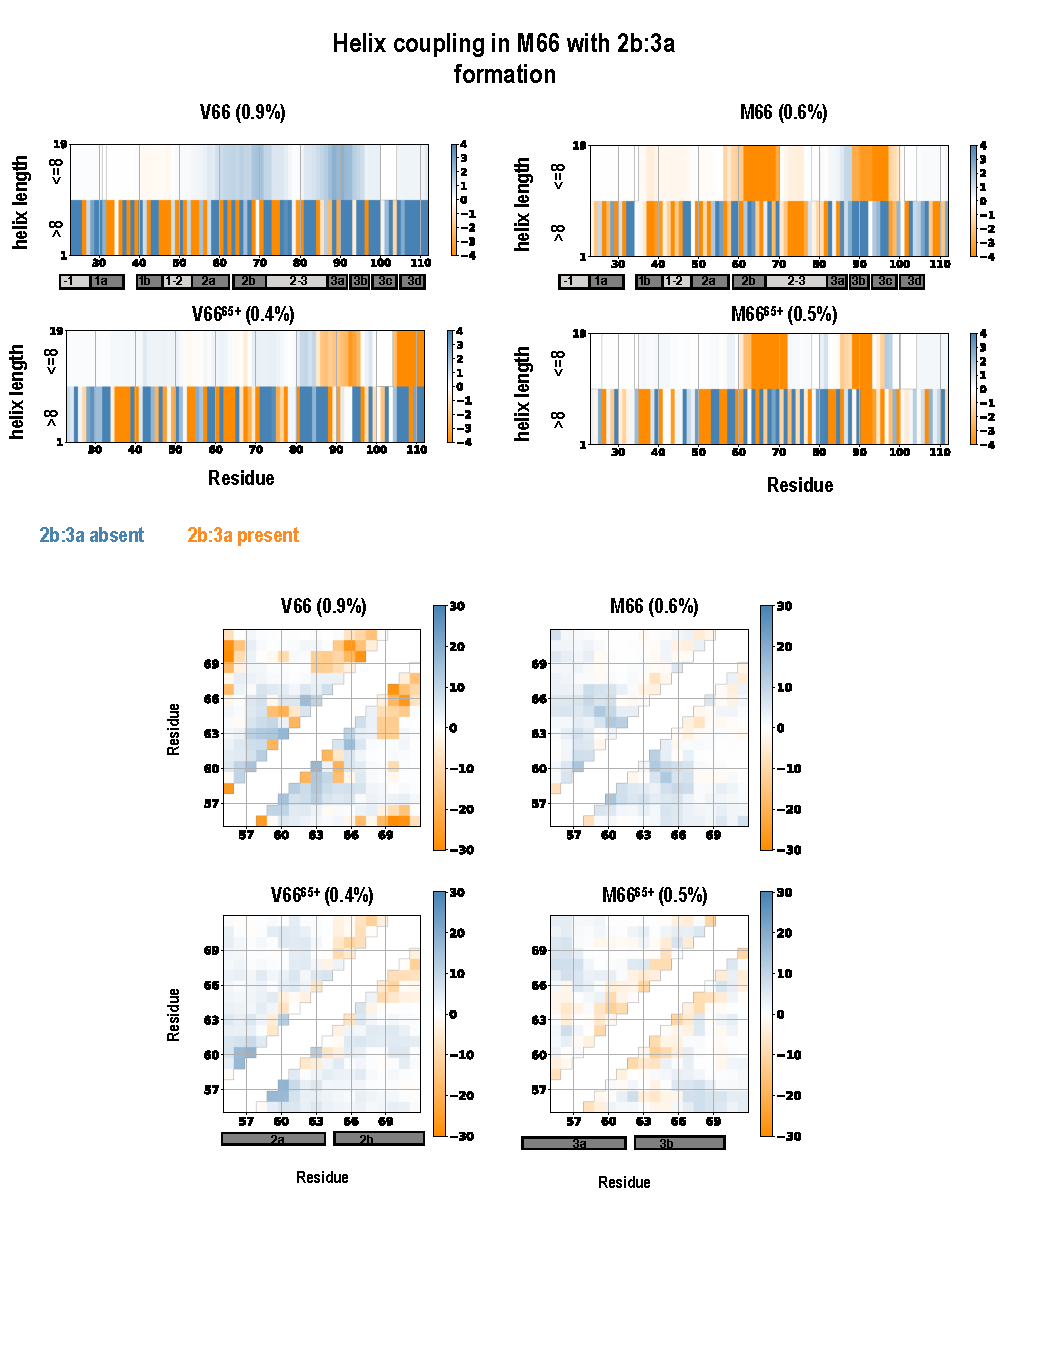
\includegraphics[scale=0.5,width=12cm,trim={0 0cm 0 0cm},clip]{../figures/coupling_1.pdf}
\caption{{\bf 2b:3a contact formation in all four simulations}
 }
\label{fig6}
\end{figure}

\begin{figure}[!ht]
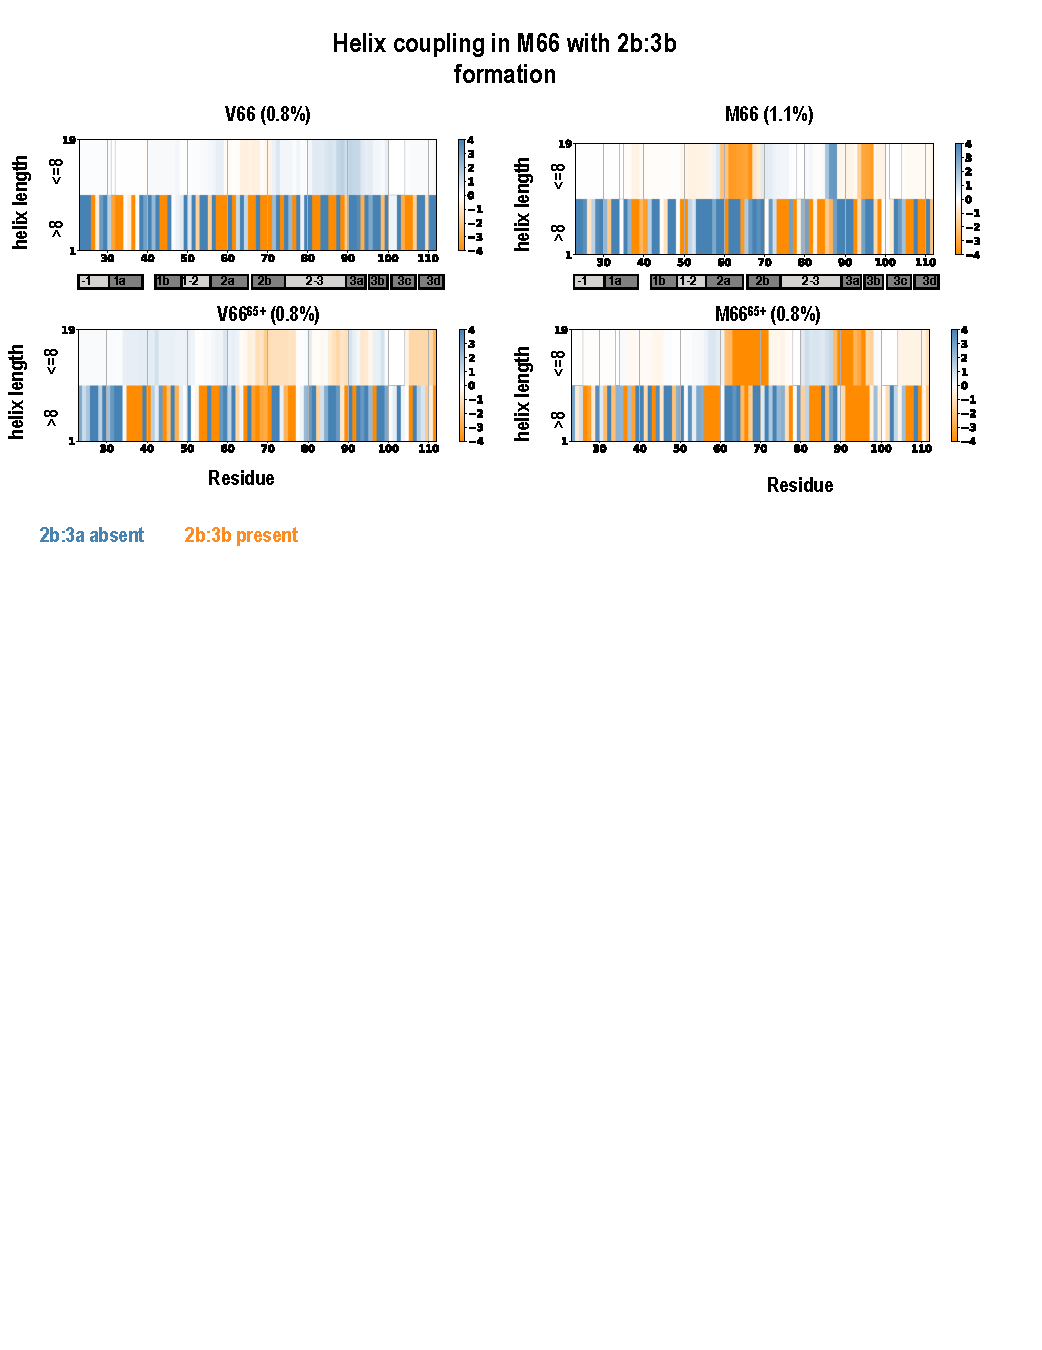
\includegraphics[scale=0.5,width=12cm,trim={0 0cm 0 0cm},clip]{../figures/coupling_3.pdf}
\caption{{\bf 2b:3a contact formation in all four simulations}
 }
\label{fig6}
\end{figure}

\begin{figure}[!ht]
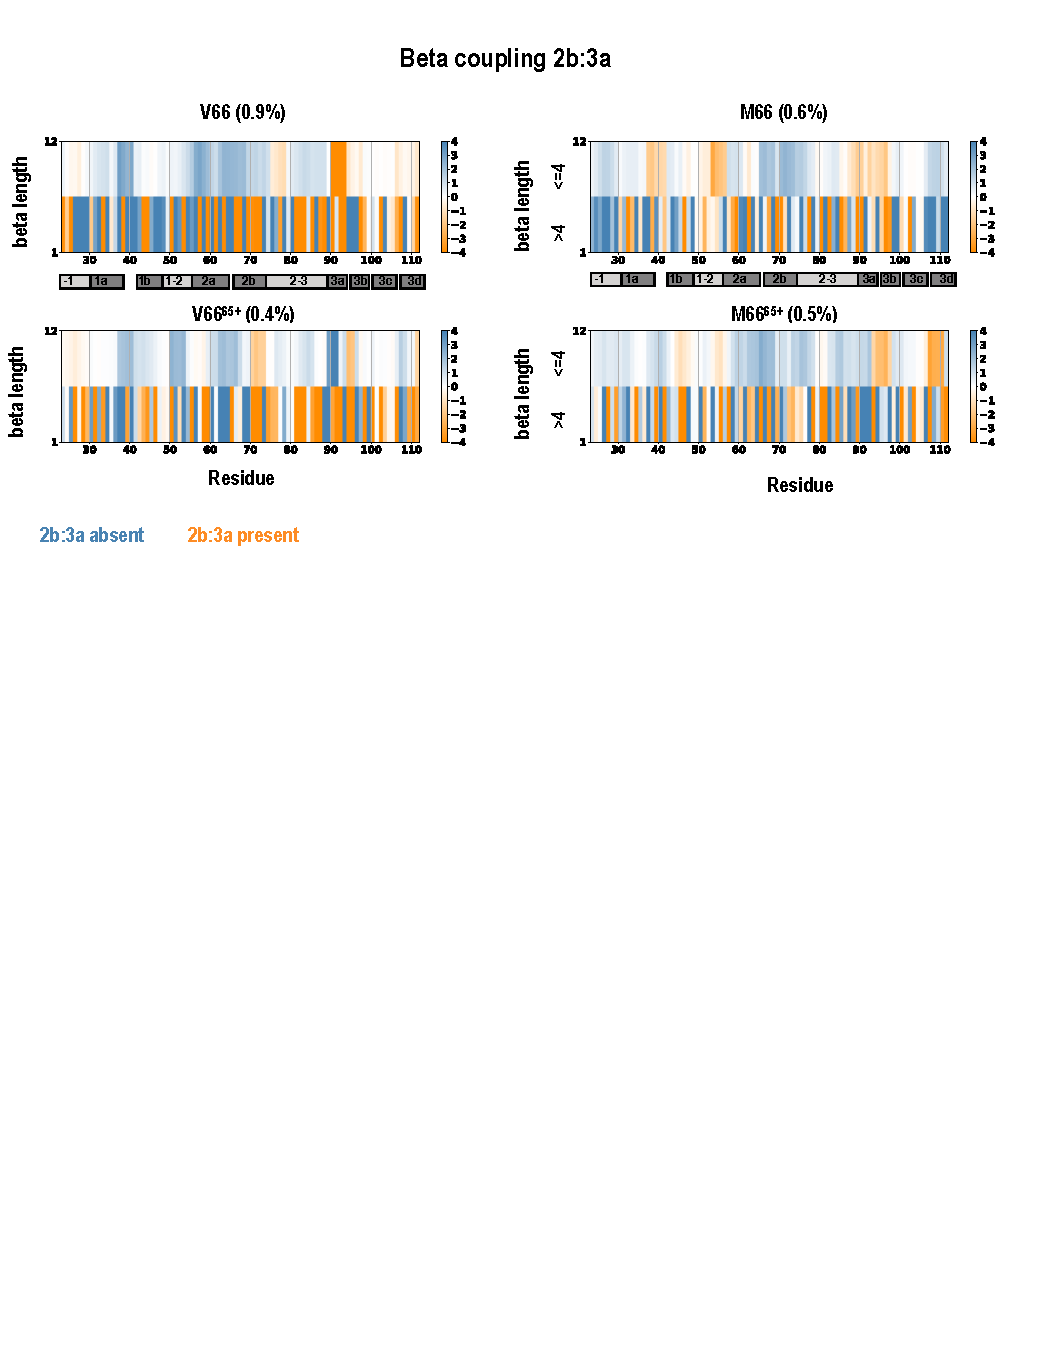
\includegraphics[scale=0.5,width=12cm,trim={0 0cm 0 0cm},clip]{../figures/coupling_4.pdf}
\caption{{\bf 2b:3a contact formation in all four simulations}
 }
\label{fig6}
\end{figure}

\begin{figure}[!ht]
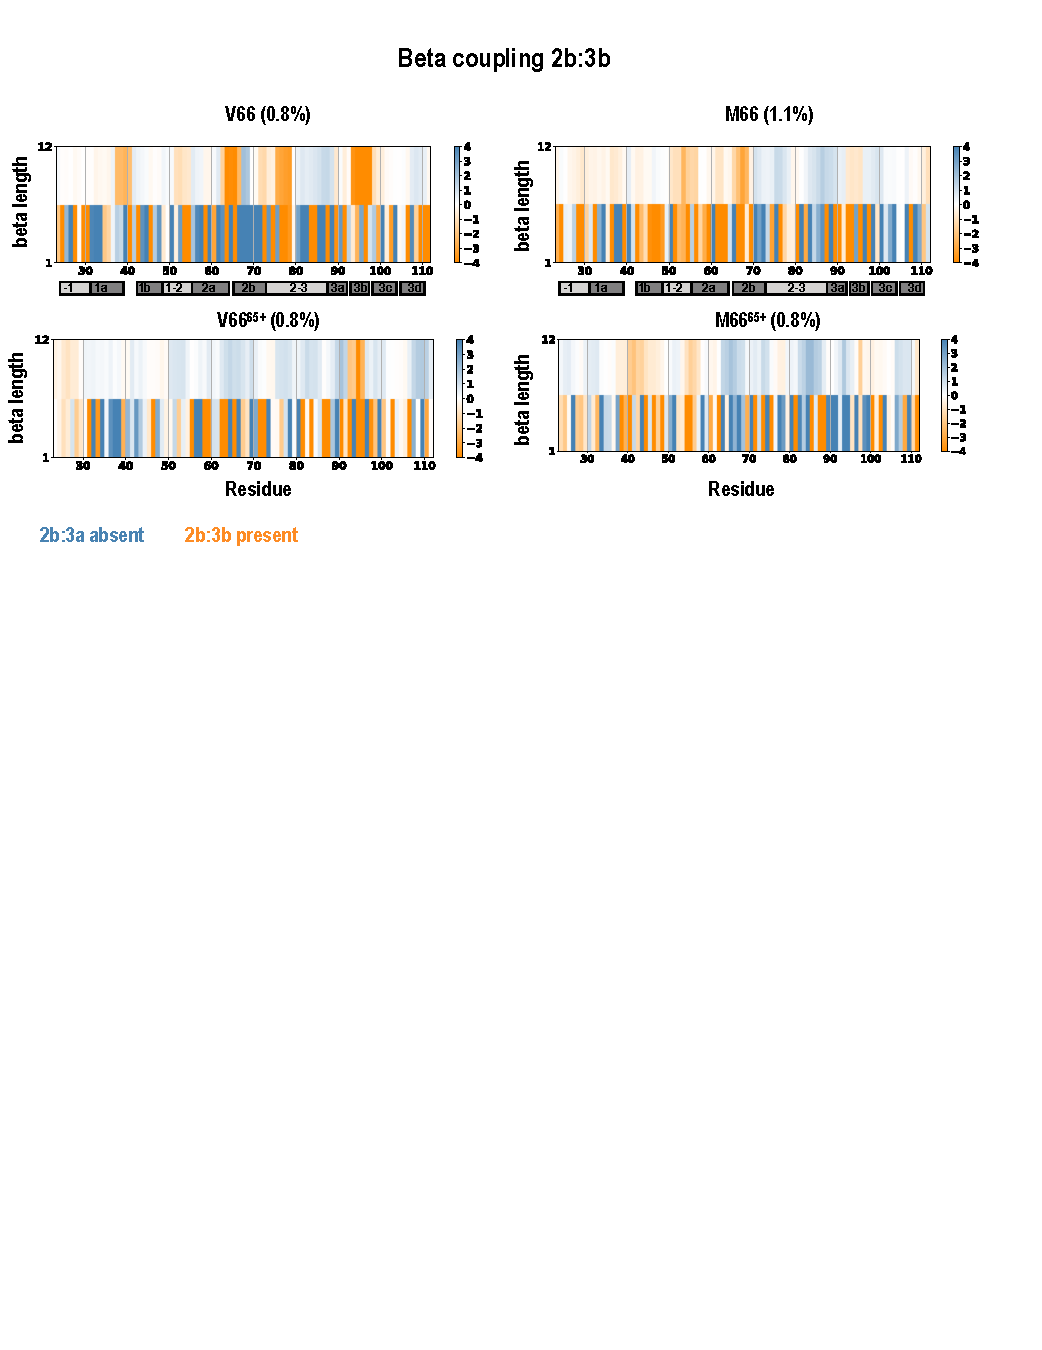
\includegraphics[scale=0.5,width=12cm,trim={0 0cm 0 0cm},clip]{../figures/coupling_5.pdf}
\caption{{\bf 2b:3a contact formation in all four simulations}
 }
\label{fig6}
\end{figure}

\begin{figure}[!ht]
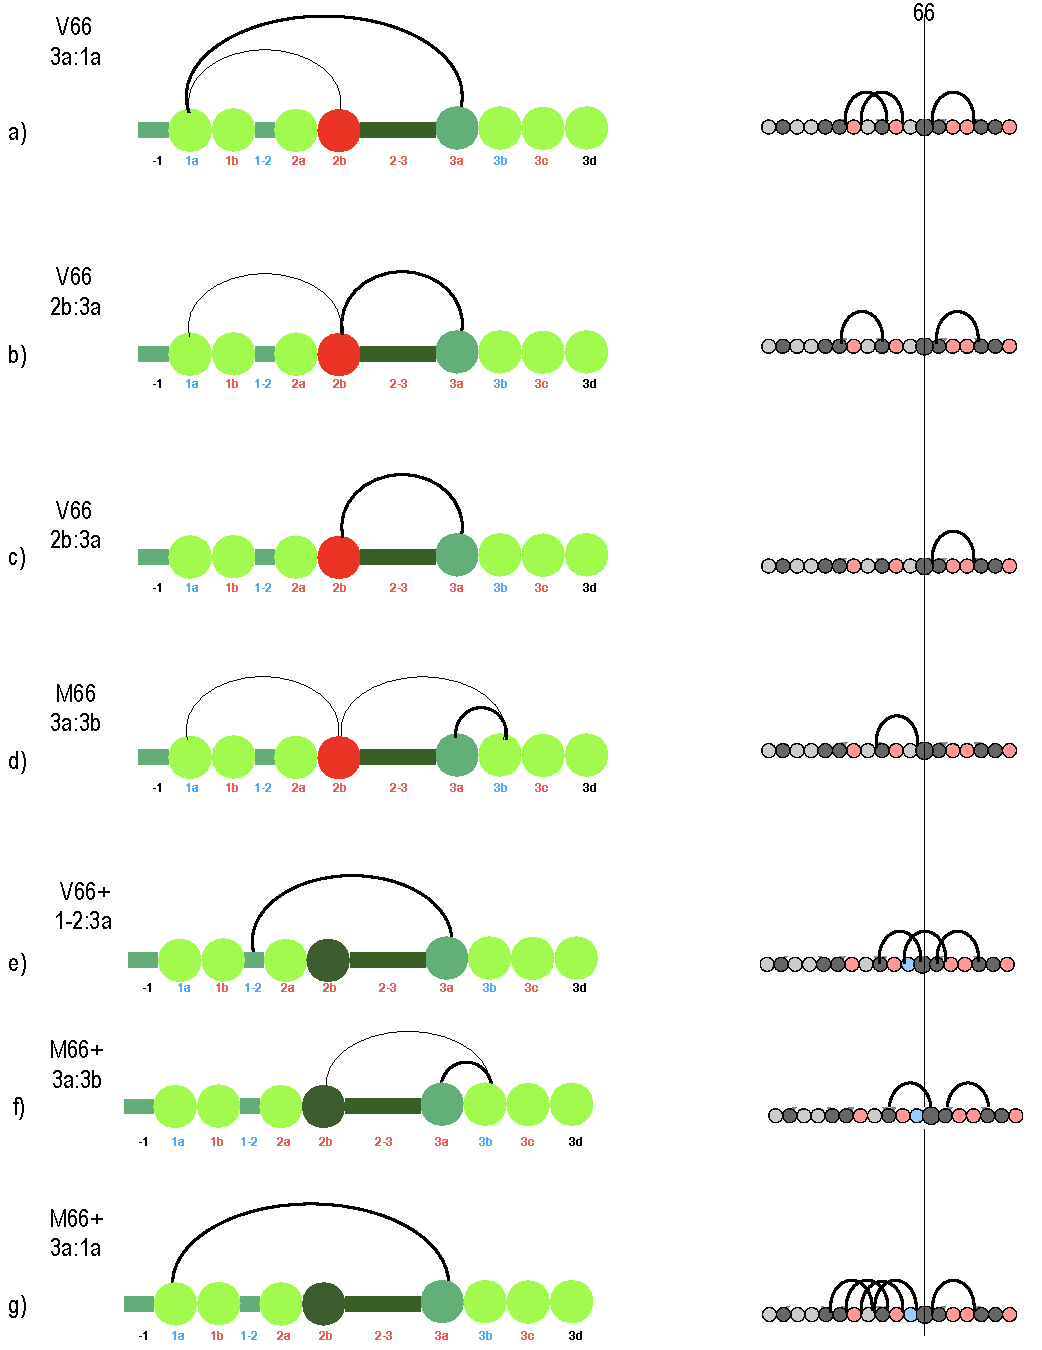
\includegraphics[scale=0.5,width=12cm,trim={0 0cm 0 0cm},clip]{../figures/fig6-1.pdf}
\caption{{\bf Long range contacts are correlated with short range contact at residues 66-69.} Left: strong inter-domain contacts formed, Right: strong intra-domain contacts formed. 
 }
\label{fig6}
\end{figure}


\begin{figure}[!ht]
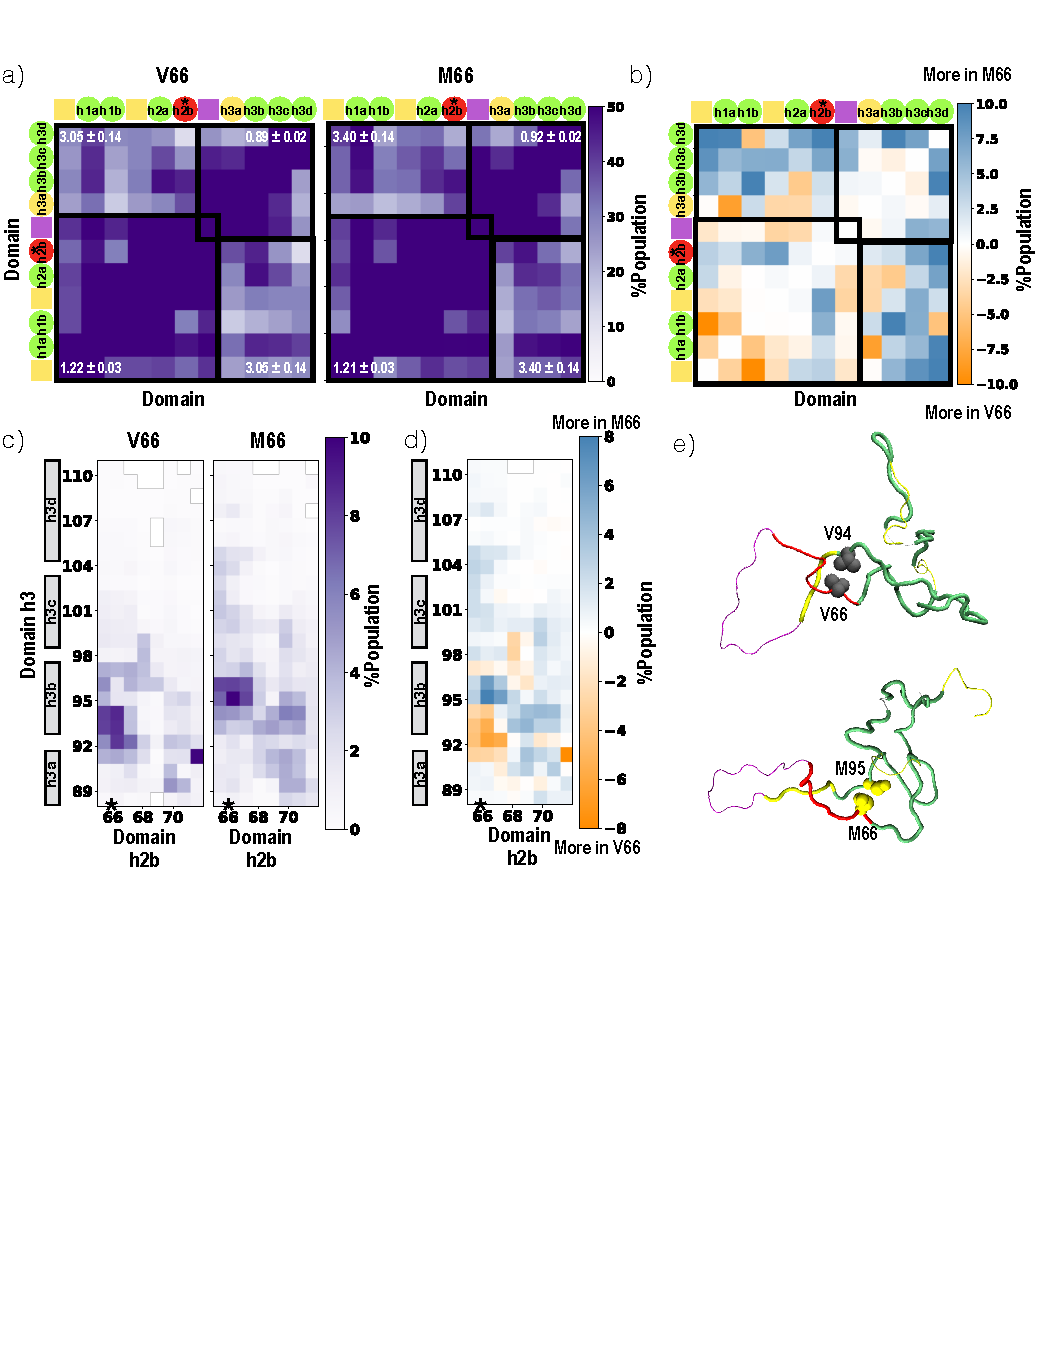
\includegraphics[scale=0.5,width=12cm,trim={0 0cm 0 0cm},clip]{../figures/fig4.pdf}
\caption{{\bf Linear networks of transient tertiary contacts.} a) The backbone tertiary-contact network is made for V66 and M66, with each residue serving as a node in the network, as described in Methods. A contact is formed if the C$\alpha$ atoms of two residues are within .85nm of each other. If the two residues forming contact are more than 24 residues apart the edge is drawn on the top of the node, otherwise the edge is drawn at the bottom of the node. Backbone interactions serve as edges between individual network nodes; the thickness  and the transparency of the edge corresponds to the strength of the contact. Contacts observed in 37 or more replicas are only visible.  Gain of protonation states looses contacts formed from x2 region for both V66 and M66.
 }
\label{fig4}
\end{figure}

%The prodomain has several well defined regions forming long-range tertiary contacts. \grace{We need to settle on one of two options : 1) defining the sticky domains according to hydrophobicity and showing that the tertiary contacts follow or 2) defining the domains from tertiary contacts and showing that they happen to be hydrophobic.}  All the four regions identified has high density of hydrophobic residues (Fig~\ref{fig1}c). It has been frequently observed that unfolded proteins form strong hydrophobic contacts ~\cite {Dobson1998}. Thus, it's not very surprising that the disordered prodomain has the presence of persistent hydrophobic contacts. \grace{Not sure about the previous - hydrophobicity is important for aggregation in general, within and among folded and misfolded proteins, it's just not very specific.  I'd like to change this remark but let's chat about it} Charges in the hydrophobic regions seem to determine the strength of contact formed between two hydrophobic regions.  x2 region, which is negatively charged forms contact with positively charged x3 region or neutral x1 region. Compact states of IDP's due to hydrophobic interactions have been observed in the past as well ~\cite {Chebaro2015, Kizilsavas2017}.


\begin{figure}[!ht]
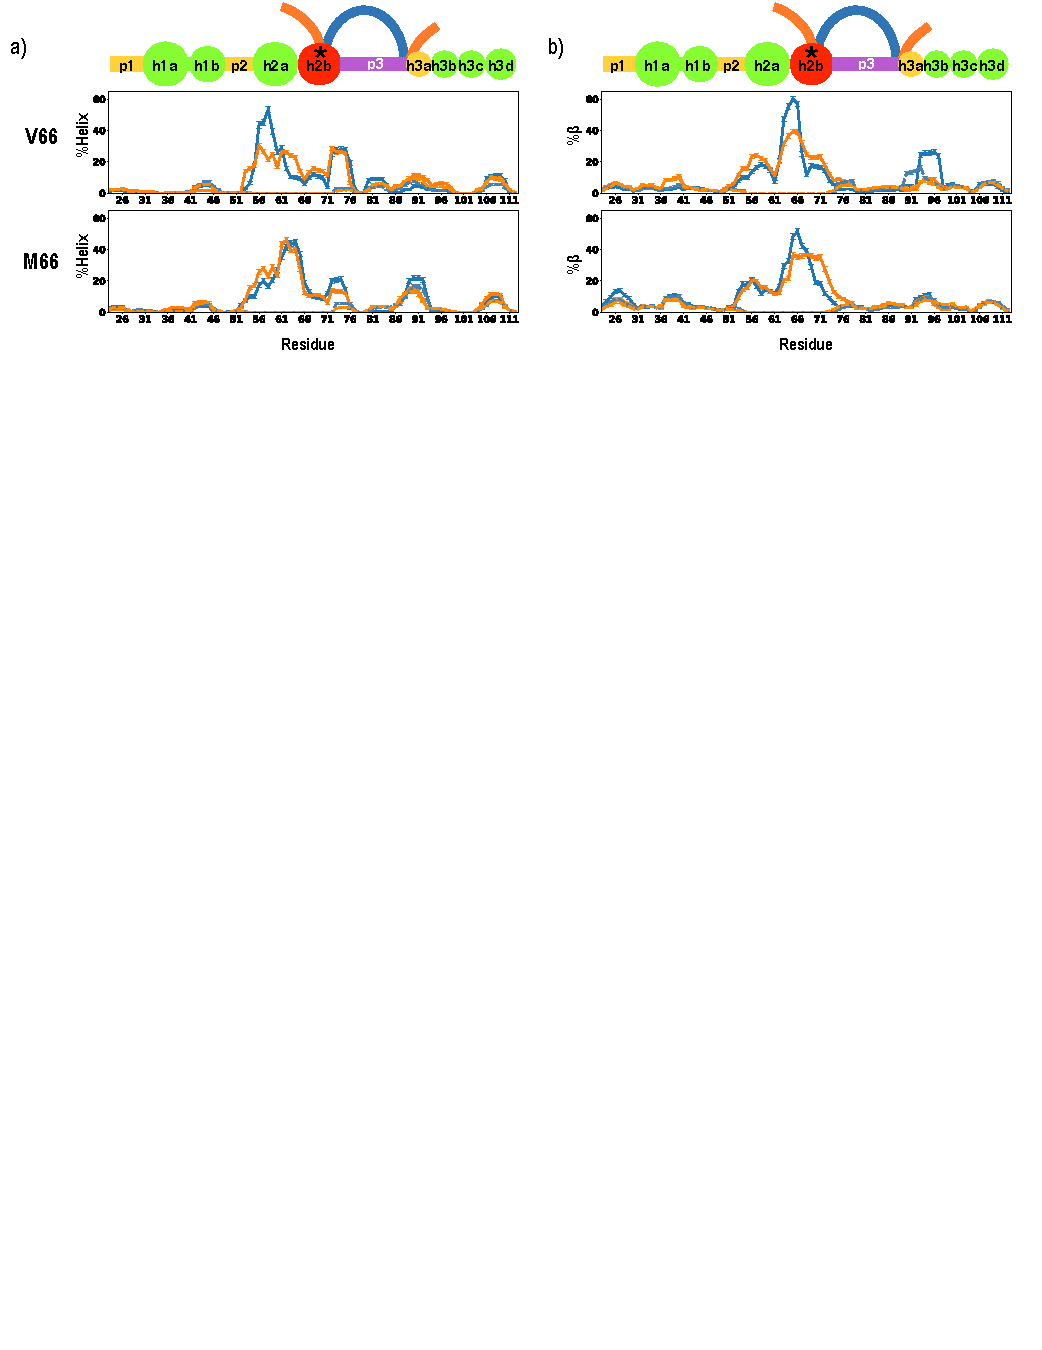
\includegraphics[scale=0.5,width=12cm,trim={0 0cm 0 0cm},clip]{../figures/fig6.pdf}
\caption{{\bf Long range contacts are correlated with short range contact at residues 63, 65, 66 or 67, 69.} Two strongest non-correlated long range contact formed in V66 a) and M66 b)Several residues near the mutation (residues E64,E68, and E69) are negatively charged. Both V66 and M66 looses salt-bridge with the gain of positive charged residue in the otherwise negatively changed region of the sequence. 
 }
\label{fig6}
\end{figure}
%\textbf{V66 collapse is driven by electrostatic contacts at center whereas M66 collapse is driven by hydrophobic contacts.} We look at the effect of Val66Met on long-range contacts. Even though the prodomain is disordered we identify loss of specific residue contact at 66. M66 and M66\textsuperscript{65+} forms strong hydrophobic contacts at residue M66-Y34 when compared with V66 and V66\textsuperscript{65+} respectively.  
%In V66, Y34 forms strong contact with residue L70. However, this hydrophobic contact is formed with simultaneous salt bridge formation between residue 27 and 72. 
%The strong hydrophobic contacts at residue 66 forms comparatively collapsed structures in M66, M66 (p) when compared with V66 and V66 (p). It has been earlier observed that  the intrinsic disorder and acidic residues keep two hydrophobic motifs from driving collapse. Instead, the most-active variants keep their aromatic residues exposed to the solvent. ~\cite {Staller2018}




\clearpage

%\section{OLD Results and discussion}

%\newcommand{\tdomain1}{\d1}
%\newcommand{\tdomain2}{d1}


%were \domain1 

%\subsubsection*{Predictions from MD trajectories {\it vs} NMR data} 
%
%In order to get accurate structural characterization of proBDNF with MD,  we did  500ns of T-REMD simulations of 30 residue fragment of V66 proBDNF with few popular ff  and water model combinations and proceed with  amber99sb*-ildn-q ~\cite{Lindorff-Larsen2010a, Hornak2006a} with Tip4p-D ~\cite {Piana2015} since it gave best agreement with experimental data obtained by NMR ~\cite{Anastasia2013} (add SI reference).  
%
%\begin{figure}[!ht]
%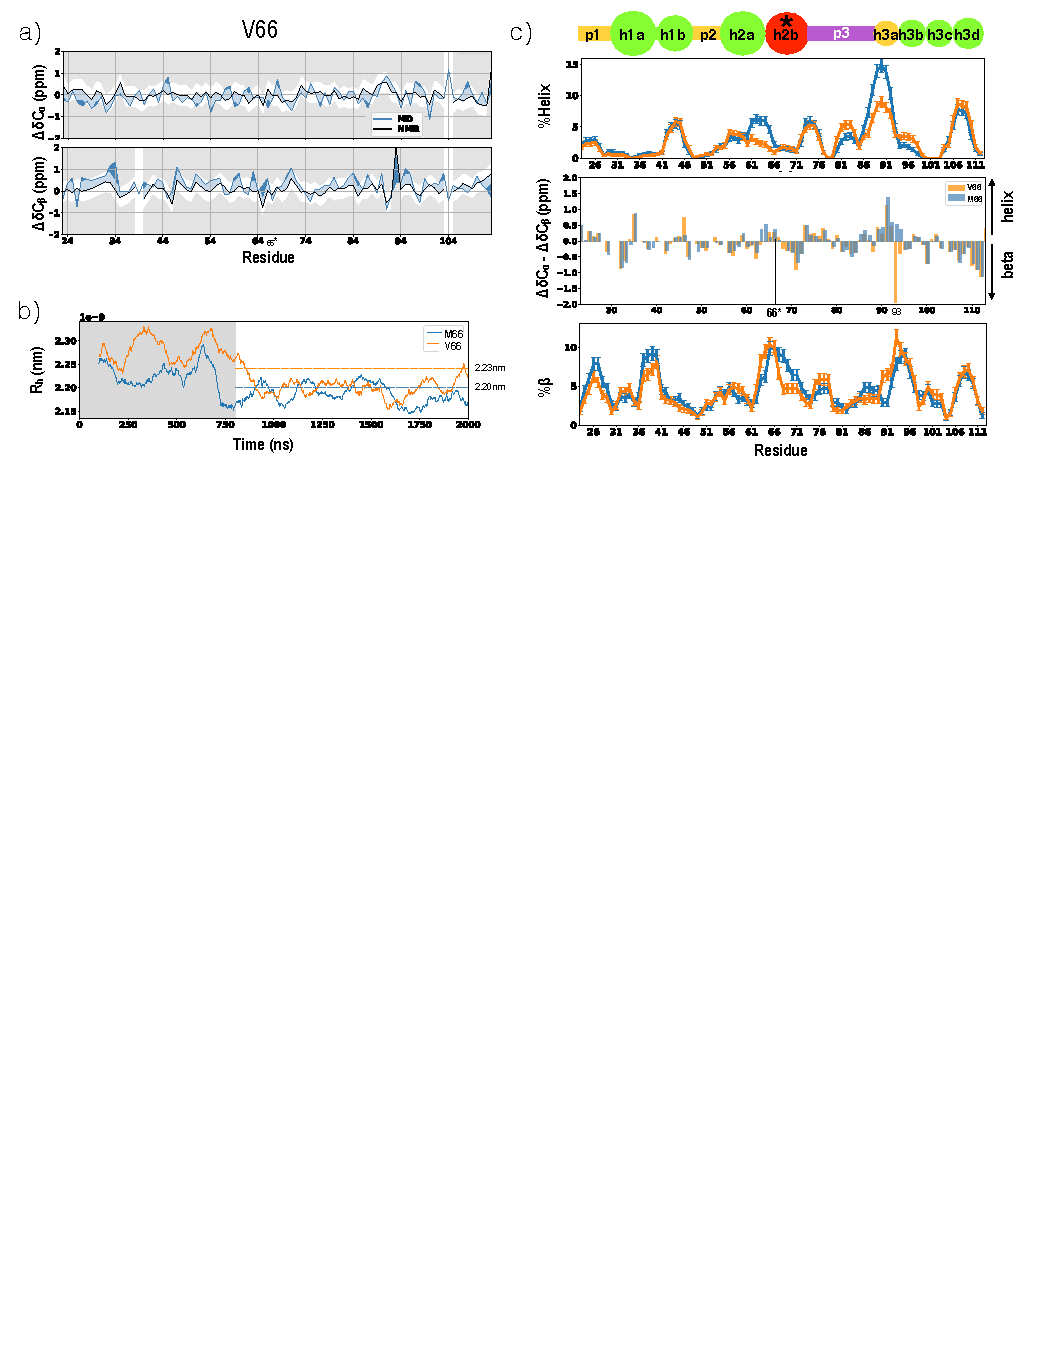
\includegraphics[scale=0.5,width=\textwidth,trim={0 0cm 0 0cm},clip]{../figures/fig2.pdf}
%\caption{{\bf Comparison of MD and NMR observables.} a) Comparison of calculated chemical shifts from MD ensembles at 300K and NMR chemical shifts from ~\cite{Anastasia2013}  at 280K,  as described in methods. b) Rh at 100 ns moving  window for V66\textsuperscript{65+} and M66\textsuperscript{65+} vs simulation time. The Rh for V66\textsuperscript{65+} and M66\textsuperscript{65+} converge after 800ns of simulation at 300K. c) STRIDE predicted secondary structure at each residue at 300K (top) and 385K (bottom).  Protonated his65 has increased tendency of forming long helix at residue 66 only for M66. The background of the plots are colored according to residue type: blue-basic, red-acidic, green-polar, white-hydrophobic. d) CA-CB secondary chemical shifts for V66 and M66 from  ~\cite{Anastasia2013}  at 280K. Positive difference indicate helical structure and negative differences indicate beta structure. Region x2 (residues 63-67) and x3 (residues 93-95) have slightly higher tendency of being helical in M66 ( marked with stars ).}
%\label{fig2} 
%\end{figure}
%%
%In order to access the validity of MD generated ensembles, we compare the MD ensembles with experimental data obtained by NMR spectroscopy and NMR diffusion measurements. Fig~\ref{fig2}a compares MD chemical shift and NMR chemical shifts. We get good agreement with NMR chemical shifts; deviations at each residue is \textless 0.5 ppm. Since the chemical shifts for V66 and M66 differ only slightly at few residues positions, we get similar chemical shifts for all 4 simulations as well (very less  \textless 0.5 ppm at each residue) (add SI reference). 
%Although there are some localized discrepancies for certain residue types(Y34, Y113, R93, R27), we get discrepancy at same residues for all four simulations. Thus, specific discrepancy is probably reflecting residual force-field inaccuracies. Consistent with intrinsic disorder, helix and $\beta$ propensity for each residue was low for both MD at 300K and NMR data at 280K. It has also been earlier observed that for IDP's with little or no secondary structure,  Amber99sb*-ildn-q with Tip4p-D gives good agreement with experimental NMR measurements. ~\cite {Robustelli2018}.
%The simulated hydrodynamic radii calculated using Hydropro ~\cite {Ortega2011} of V66 (2.21 nm) and M66 (2.18 nm) are in excellent agreement with the experimental values (2.24 nm and 2.20 nm respectively) (Fig~\ref{fig2}b). This method has been used earlier to validate IDP ensembles ~\cite {Rauscher2015, Meng2018} and it confirms that the overall dimensions of the protein is reasonable.  This is not surprising as Tip4p-D has been optimized to reproduce the dimensions of disordered proteins ~\cite {Piana2015, Robustelli2018}. 
%
%Most of the IDP simulations studies have been performed on smaller IDP fragments (residues 3-42) ~\cite{Henriques, Rauscher2017, Meng2018} . We performed the explicit solvent replica simulations of 91 residues, which was computationally challenging and thus we carefully accessed the convergence of our simulations. All replicas were able to diffuse in the temperature range 300K to 385K (replica round trip number \textgreater 7) (Fig S1). The Rg for V66 and M66 converge after 800ns of simulation at 300K (Fig~\ref{fig2}b). We discarded the first 800 ns of the trajectories as conformational equilibration. The Rg distribution of all four simulations are unimodal (Fig~\ref{fig4}b). 
%
%
%NMR studies ~\cite{Anastasia2013}  found increase in helical tendency for M66 at region x2 (residues 64,65,66) and region x3 (residues 90 to 94) ( marked with stars ) and decrease in helical tendency at region x1 (Fig~\ref{fig2}c). To look into the effect of mutation on residual secondary structure, we compare the helix tendency at every residue for each of the four simulation (Fig~\ref{fig4}c). Consistent with NMR experiments, M66 and M66\textsuperscript{65+} has increased tendency of forming $\alpha$-helix at region x1 when compared with V66 and V66\textsuperscript{65+}(Fig~\ref{fig2}c). \grace{for comparing MD and NMR secondary structure most likely d2D calculations and comparisons will make more sense ?} 
%%todo for comparing MD and NMR secondary structure I need to do d2D calcualtions


%\subsubsection*{Both mutation at residue 66 and protonation at 65 increases helix formation at residue 66}
%
%Consistent with NMR data ~\cite{Anastasia2013}, both Val66Met and Val\textsuperscript{65+}66Met\textsuperscript{65+} changes the frequency of long helix ( \textgreater 6 residues)  formed at region x2 and x3 and beta sheets ( \textgreater 4 residues) at region x3 (Fig~\ref{fig3}a). However, how the mutation causes this differential chemical shifts is not known. 
%
%To get more insight at the helix formed at 66, we look at the population of each helix length formed at 66 (Fig~\ref{fig3}b). Only M66 and not V66 has long helix formation at residues 59-67 (9 residues). Additionally, M66\textsuperscript{65+} forms even longer helix 62- 71 (10 residues).

%\begin{figure}[!ht]
%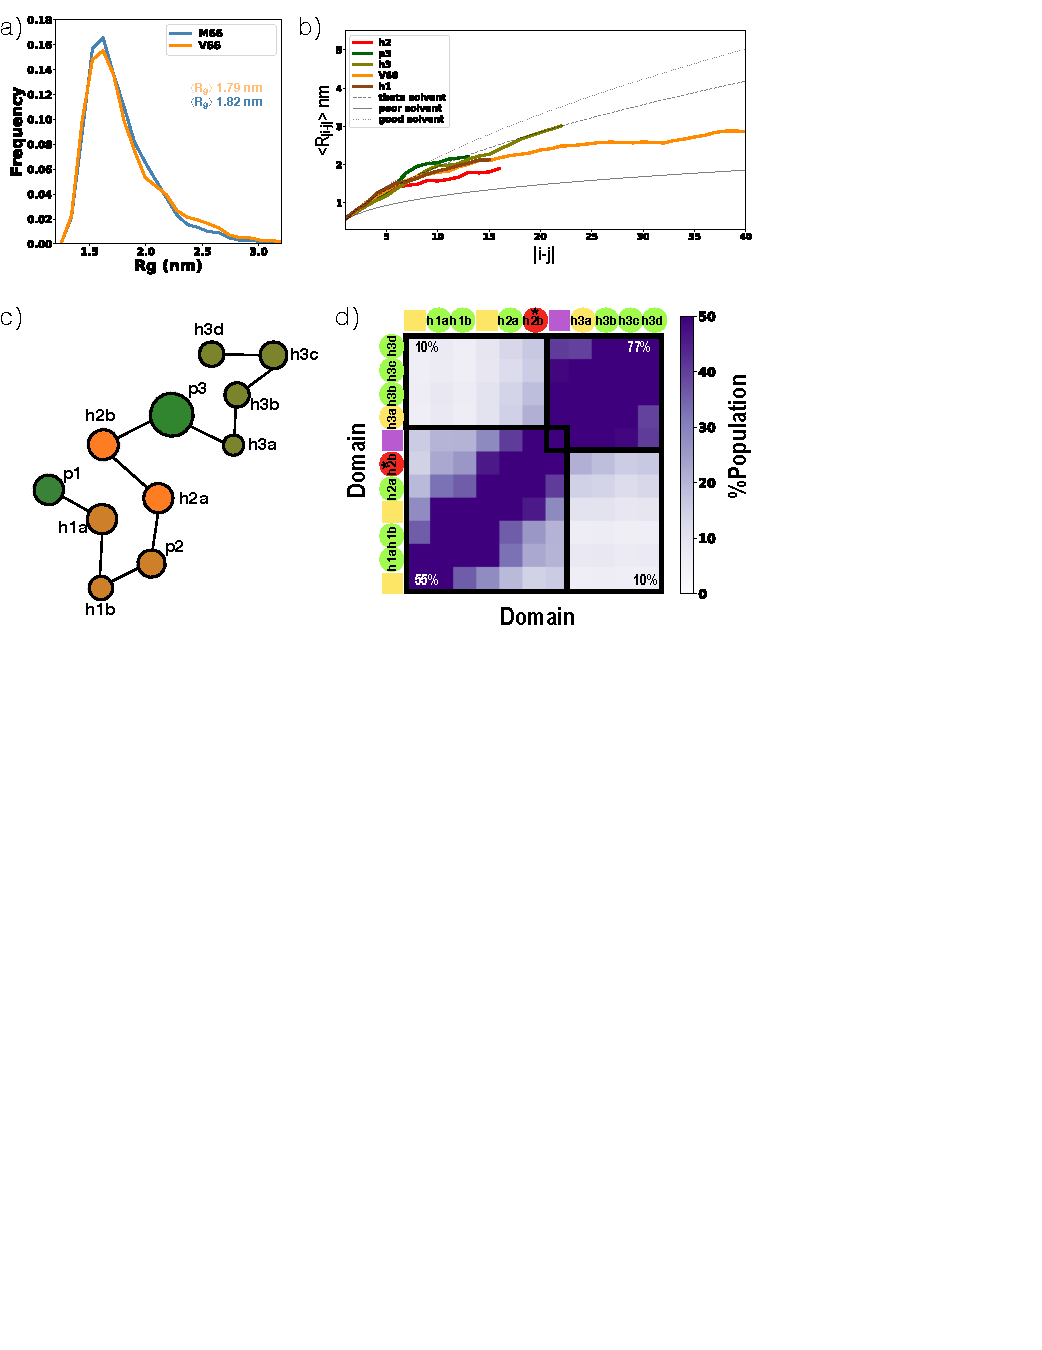
\includegraphics[scale=0.5,width=\textwidth,trim={0 0cm 0 0cm},clip]{../figures/fig3.pdf}
%
%\caption{{\bf Simulation predicted secondary structure properties.}
%a) Difference in helix length (top) and beta length (bottom) for each residue. In agreement with the experiment, we find higher tendency of forming longer helix at regions x2 and x3. V66 has higher tendency of forming beta at region x3.  b) Helix length distribution at each residue when 66 is in the helix region of ramachandran map (methods) }
%
%\label{fig3} 
%\end{figure}

%\subsubsection*{Most long range contacts occur among 4 well-defined regions} 
%
%Conventional contact maps provided little useful insight into tertiary structure for either forms of the protein, which was consistent with the intrinsic disorder and frequent transient interactions among neutral side-chains. Identification of contact residues yielded several persistent, weak long-range interactions at 300K for both sequences, which can be represented along a single axis (Fig~\ref{fig4}). 
%
%\begin{figure}[!ht]
%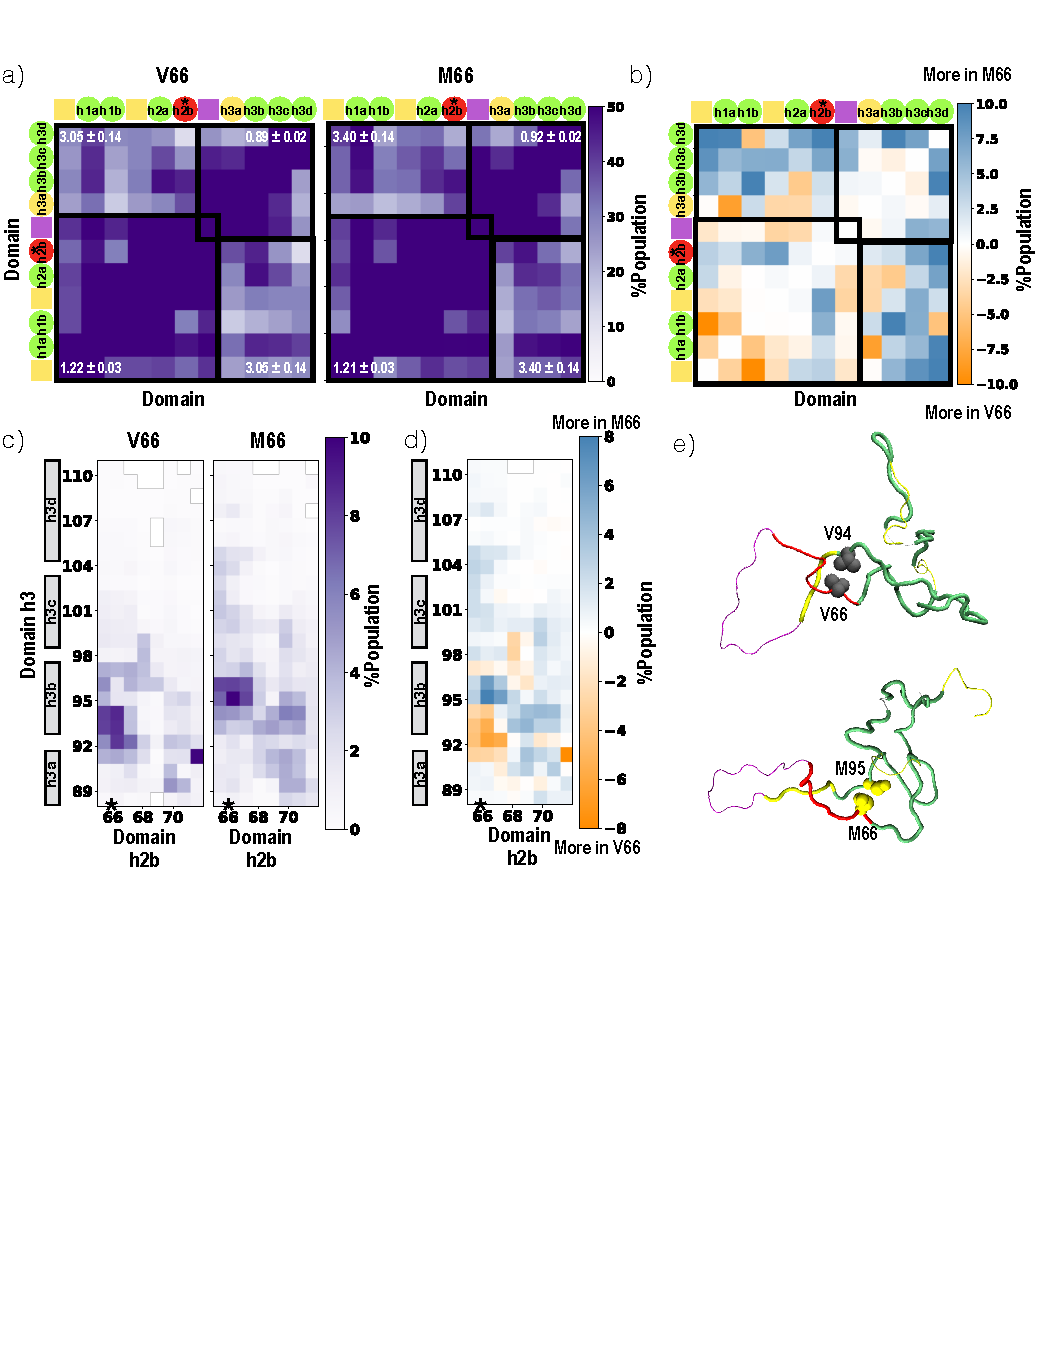
\includegraphics[scale=0.5,width=12cm,trim={0 0cm 0 0cm},clip]{../figures/fig4.pdf}
%\caption{{\bf Linear networks of transient tertiary contacts.} a) The backbone tertiary-contact network is made for V66 and M66, with each residue serving as a node in the network, as described in Methods. A contact is formed if the C$\alpha$ atoms of two residues are within .85nm of each other. If the two residues forming contact are more than 24 residues apart the edge is drawn on the top of the node, otherwise the edge is drawn at the bottom of the node. Backbone interactions serve as edges between individual network nodes; the thickness  and the transparency of the edge corresponds to the strength of the contact. Contacts observed in 37 or more replicas are only visible.  Gain of protonation states looses contacts formed from x2 region for both V66 and M66.
% }
%\label{fig4}
%\end{figure}
%
%Prodomain has well defined regions forming long-range tertiary contacts. All the four regions identified has high density of hydrophobic residues (Fig~\ref{fig1}c). It has been frequently observed that unfolded proteins form strong hydrophobic contacts ~\cite {Dobson1998}. Thus, it's not very surprising that the disordered prodomain has the presence of persistent hydrophobic contacts. Charges in the hydrophobic regions seem to determine the strength of contact formed between two hydrophobic regions.  x2 region, which is negatively charged forms contact with positively charged x3 region or neutral x1 region. Compact states of IDP's due to hydrophobic interactions have been observed in the past as well ~\cite {Chebaro2015, Kizilsavas2017}.





%\subsubsection{Why does Val66Met increases helix formation at residue 66}



%\begin{figure}[!ht]
%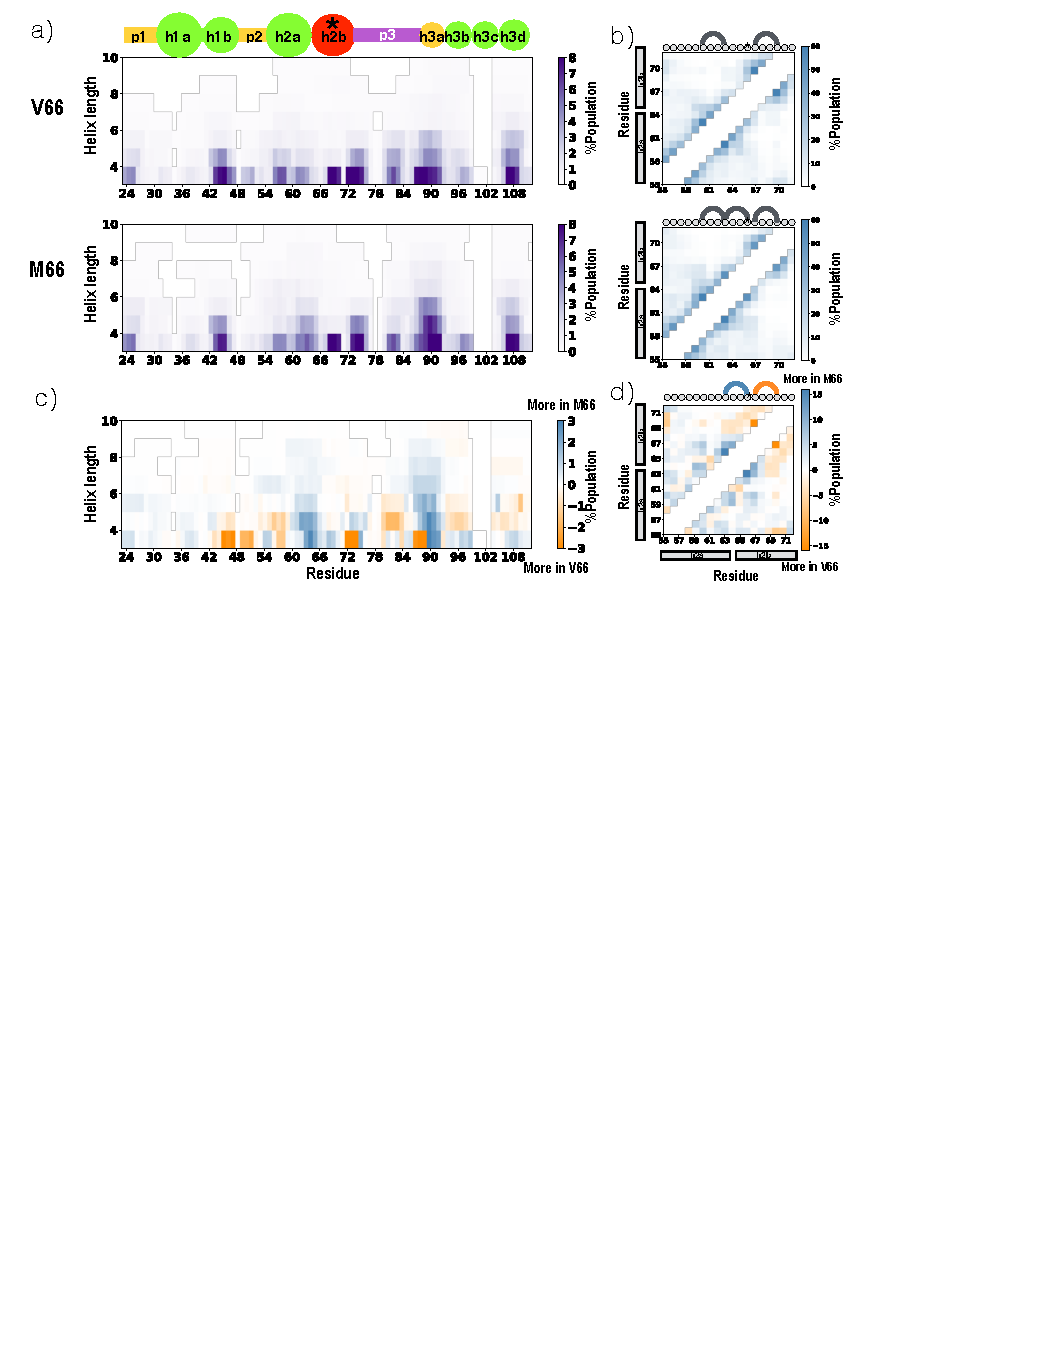
\includegraphics[scale=0.5,width=\textwidth,trim={0 0cm 0 0cm},clip]{../figures/fig5.pdf}
%
%\pagebreak
%
%\caption{{\bf Contacts formed at residue i and i-3.}
%Weight of contact formed at every residue pair separated with two residues (residue i and i-3) for V66 and M66 (top).  Difference in V66 and M66 residue pair contacts(bottom). M66 forms strong contact at residue M66:F63, whereas V66 forms strong contact at residue I67:L70.}
%
%
%\label{fig5} 
%\end{figure}
%Increased helix formation in M66 is contributed by two factors. 
%a) Reduced entropic cost of helix formation in M66 when compared with V66. Creamer et. al. ranked the entropic cost of helix formation for apolar side chains using simulations of a (Ala)\textsubscript{8} sequence with the 'guest' amino acid at the center and reported higher entropic cost helix formation for Valine when compared with Methionine \cite{Creamer1992}. 
%
%b) Helix stabilization in M66 by preferential contact formed between M66:F63. We looked at the weight of the contact formed at every residue pair separated with two residues (Fig~\ref{fig5}). Either two hydrophobic residues (L43:V46, A60:F63,A87:Y90 ) or  two residues with opposite charge (E73:K76), commonly form strong contacts (\textgreater 65\%) for both V66 and M66. Additionally, M66 forms strong contact at residue M66:F63, whereas V66 forms strong contact at residue I67:L70. A previous study from Faure et al ~\cite {Faure2008} analyzed the frequency of two amino acids contact within 1230 protein chains from Protein DataBank (PDB) and found that Methionine (M) has also a strong affinity with Phenylalanine (F) and itself.
%
%Protonated histidine favors longer helical structure at residue 66 due to helix favored salt-bridge formation  Glu61\textsuperscript{65+} and Hip65-GLU69. Thus, addition of positive charged residue in the otherwise negatively charged region supports helix formation. 
%
%We also look at the temperature dependence of helical structure in prodomain. At 385K, the helix at residue 66 increases (\textgreater 2\%) for all V66, M66, V66\textsuperscript{65+}, but M66\textsuperscript{65+} has strongest preference (\textgreater 5\%) (Fig~\ref{fig4}c). Thus,  increased hydrophobic interaction with temperature (F63:M66) along with reduced electrostatic repulsion (H65:E69) in M66\textsuperscript{65+} favors helix formation.

%\newpage
%\subsubsection{How does Val66Met changes long range pairing}
%
%We observe few long-range contacts with significant differences in V66 and M66 with p  \textless  0.0001. \grace {The cross-over N is \~15 frames ?} . We find that the differences we observe in long-range contacts are strongly correlated with concats at residue 66,67 (i) and (i-3).
%
%\begin{figure}[!ht]
%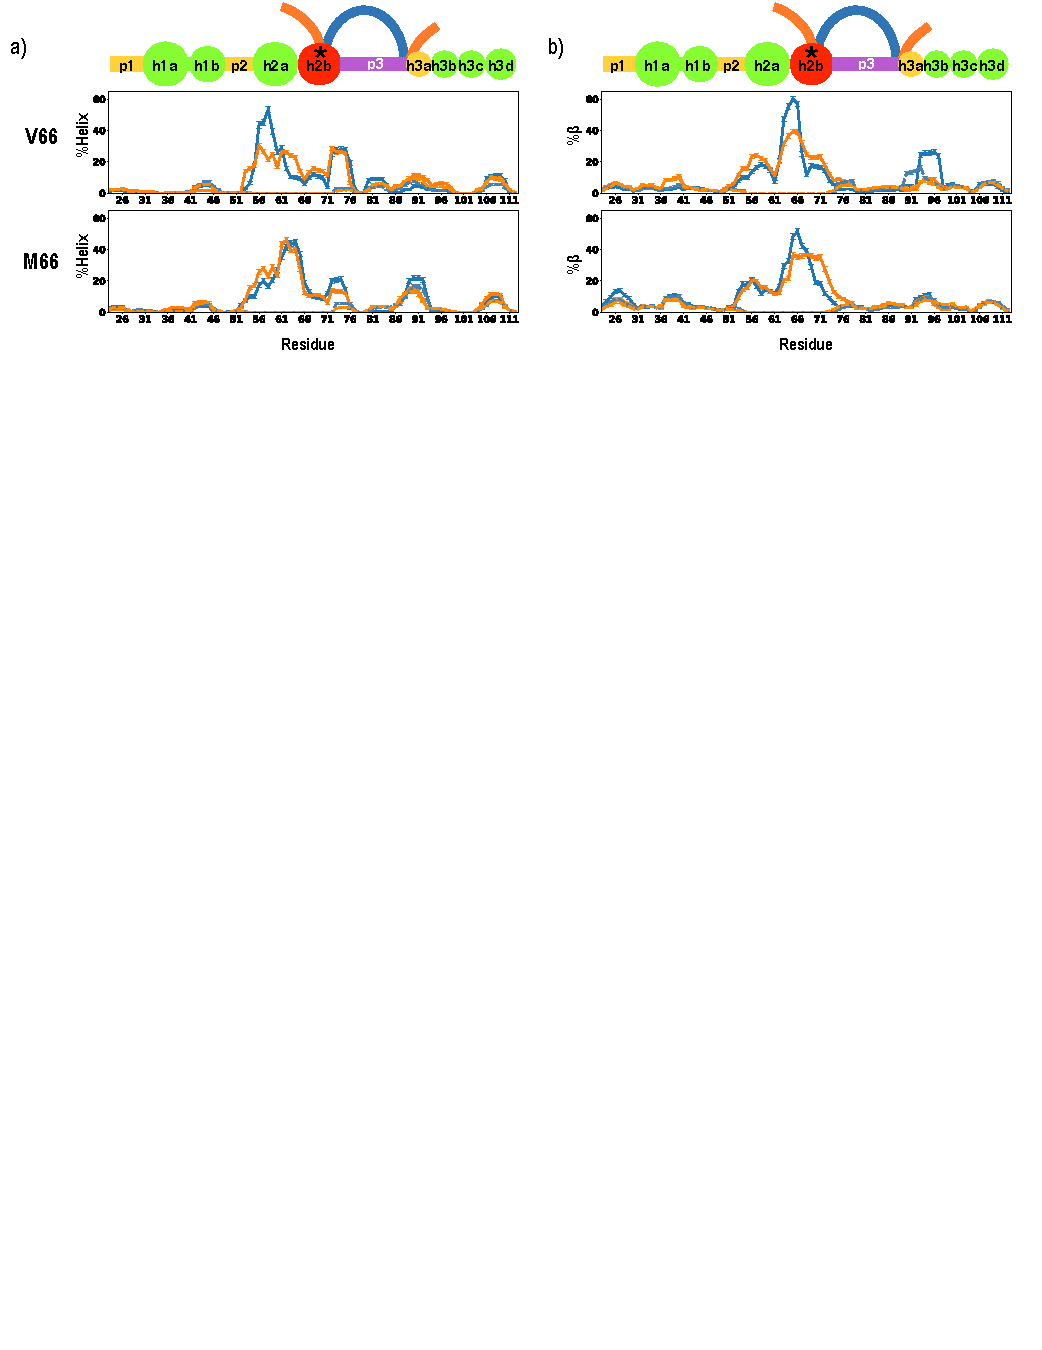
\includegraphics[scale=0.5,width=12cm,trim={0 0cm 0 0cm},clip]{../figures/fig6.pdf}
%\caption{{\bf Long range contacts are correlated with short range contact at residues 63, 65, 66 or 67, 69.} Two strongest non-correlated long range contact formed in V66 a) and M66 b). 
% }
%\label{fig6}
%\end{figure}

%\textbf{V66 collapse is driven by electrostatic contacts at center whereas M66 collapse is driven by hydrophobic contacts.} We look at the effect of Val66Met on long-range contacts. Even though the prodomain is disordered we identify loss of specific residue contact at 66. M66 and M66\textsuperscript{65+} forms strong hydrophobic contacts at residue M66-Y34 when compared with V66 and V66\textsuperscript{65+} respectively.  
%In V66, Y34 forms strong contact with residue L70. However, this hydrophobic contact is formed with simultaneous salt bridge formation between residue 27 and 72. 
%The strong hydrophobic contacts at residue 66 forms comparatively collapsed structures in M66, M66 (p) when compared with V66 and V66 (p). It has been earlier observed that  the intrinsic disorder and acidic residues keep two hydrophobic motifs from driving collapse. Instead, the most-active variants keep their aromatic residues exposed to the solvent. ~\cite {Staller2018}

%\newpage
%\subsubsection{How does Val66Met changes long range pairing when protonated at residue 65}
%
%\begin{figure}[!ht]
%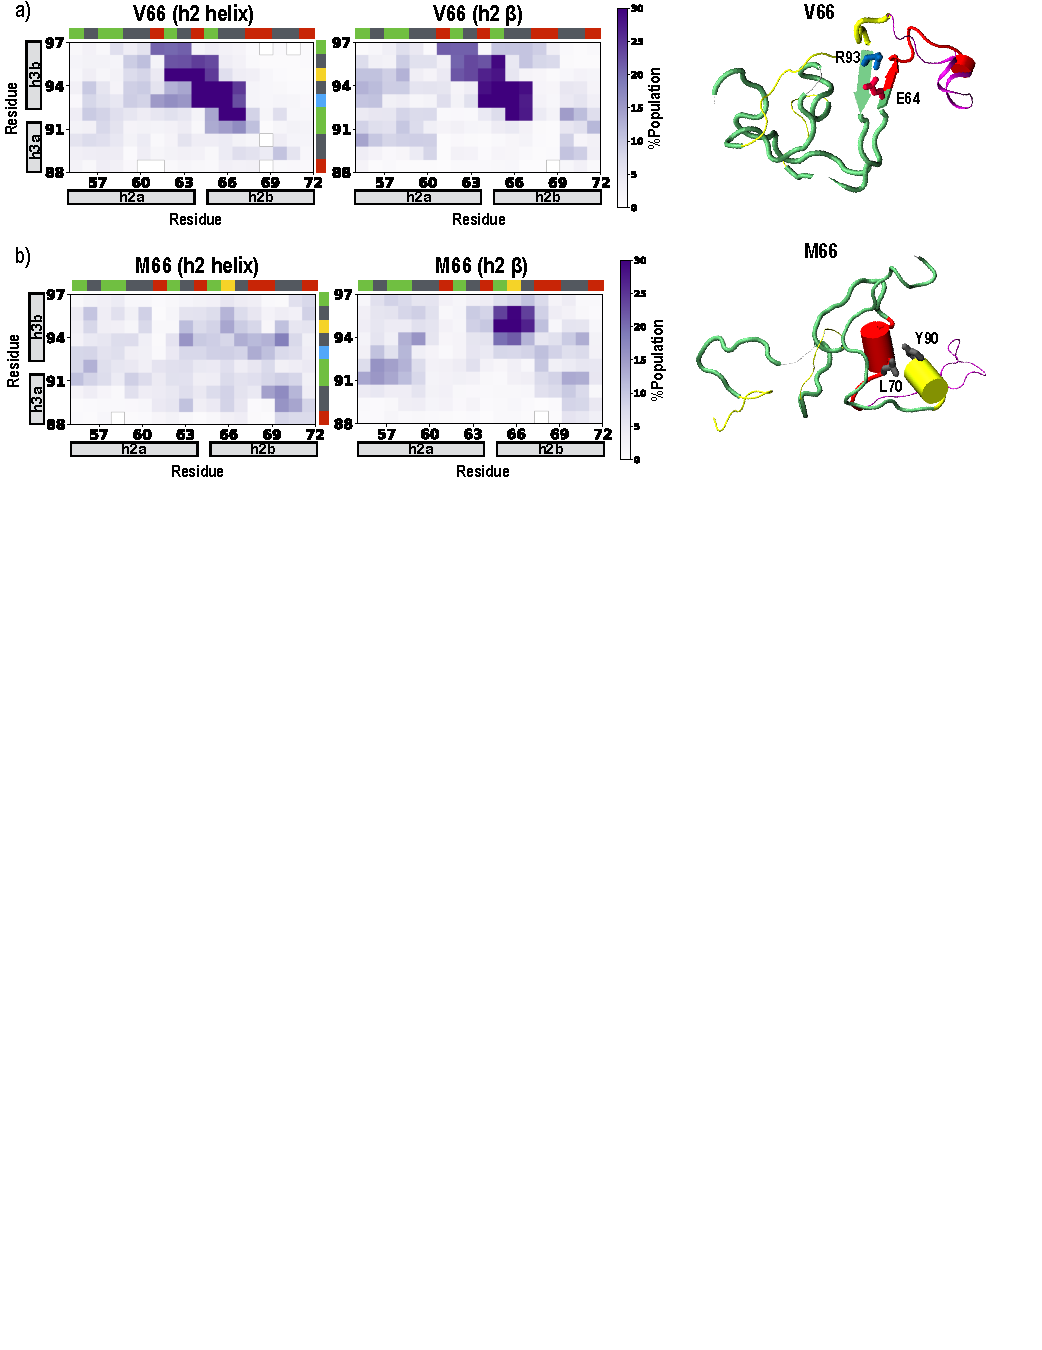
\includegraphics[scale=0.5,width=12cm,trim={0 0cm 0 0cm},clip]{../figures/fig7.pdf}
%\caption{{\bf Long range contacts are correlated with short range contact at residues 63, 65, 66 or 67, 69.} Two strongest non-correlated long range contact formed in V66 a) and M66 b). 
% }
%\label{fig7}
%\end{figure}

%\subsubsection{M66 supports helix formation at residue 93}
%
%We next examined the increased helix tendency at residue 93 from Val66Met substitution. We find structures forming helix at 93 are in contact with residue 66 in at-least 25\% of it's population in M66\textsuperscript{65+} (Fig~\ref{fig6}). The gain of this residue specific interaction in M66, probably increases helix formation at 93 when compared with V66. 
%
%\begin{figure}[!ht]
%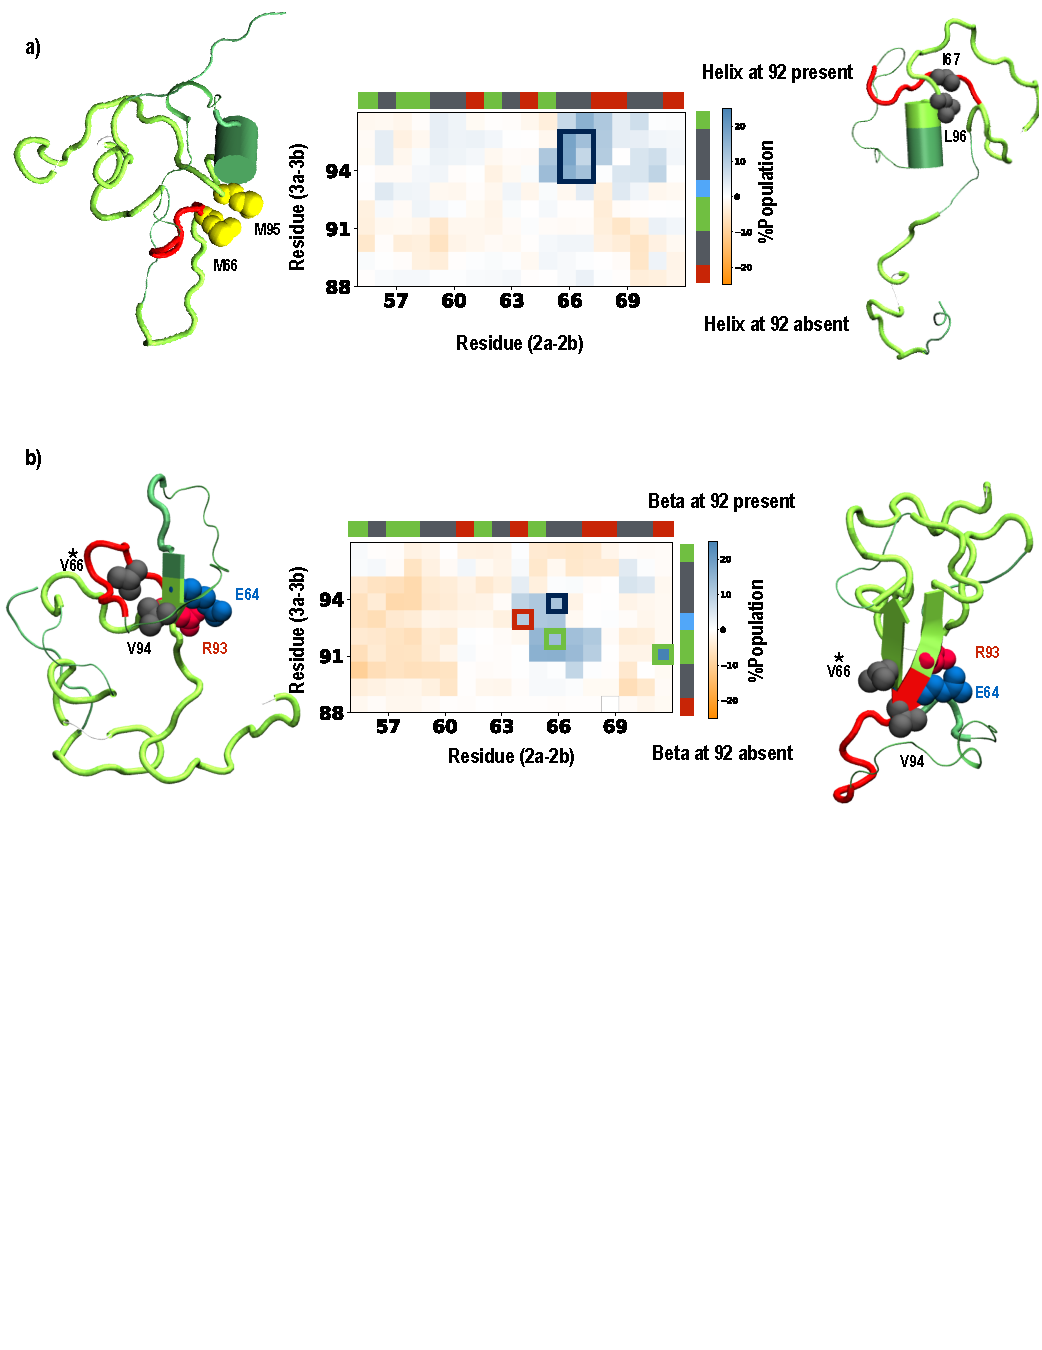
\includegraphics[scale=0.5,width=\textwidth,trim={0 0cm 0 0cm},clip]{../figures/fig8.pdf}
%
%\caption{{\bf Simulation predicted helical structure and it's comparison with experiments.} }
%
%\label{fig8} 
%\end{figure}


%\textbf{Only Val66 and not Met66 forms long beta sheet structures at residue 66 and 93.} We next examined the backbone contacts formed between residues.
%% Hip65 reduces beta sheet tendency at residue 66 for both V and M form (Fig~\ref{fig5}a). This could be due to gain of helix at 66 in Hip65 form or due to loss of sheet structures which involved salt-bridge formation at 64. 
%V66 and M66 forms differential backbone contact at residue 66 (Fig~\ref{fig5}a). V66 forms beta sheet structures with residue 92. This is also consistent with NMR observation ~\cite{Anastasia2013}  , where Val66Met changes CS at residue 93 (Fig~\ref{fig8}a) . 
%We further test if the beta sheet structures at residue 66-95 in V66 is more favored in V66 than in M66 and is not a limitation of simulation convergence. To verify this observation, we performed simulations with backbone restraints of 1Kj/mole/nm2 of a V66 frame having beta sheet structures at residue 66-95 with Val66 mutated to Met. We find that M66 has higher loss in entropy at 93 (Fig~\ref{fig5}b). Additionally, 66-92 beta structures forms 64-93 salt bridge simultaneously in V66(Fig~\ref{fig5}c). In our restrained simulations M66 has 50\% less probability of forming salt-bridge at residue 64-93 (Fig~\ref{fig5}d). This result suggests that beta at 66-95 is less favored in M66 due to higher entropic and energetic cost. 




\section*{Materials and Methods}

\subsection*{System setup} To account for differences in starting coil conformation, we included six unique structures to represent residues 23-113 of BDNF prodomain.  All structures were built using I-Tasser ~\cite{Yang2014,Roy2010,Bioinformatics}, Robetta and Modeller ~\cite{Sali1993a}, and all were simulated in a water box at 600K for 50 ns at a constant volume. From the six resulting trajectories, 10 structures with correct proline isomers were selected (based on at least 3ps time interval); in total, our study included 60 unique prodomain structures. All structures were cooled to 300K for 1ns, while prolines were restrained in trans-conformation. M66 replicas were generated by substituting Met for Val at residue 66. Each V66 and M66 replica was placed in a dodecahedron water box with 25,000 TIP3P ~\cite {Jorgensen1983} water molecules and a 0.15M salt concentration (NaCl) for a total system size of approximately 75,000 atoms. The same volume for each replica was ensured by fixing the simulation box of each replica to the average box size (10.2 nm).

\subsubsection*{Molecular Dynamics Simulation} All simulations used the amber99SB-ILDN force field\cite{Lindorff-Larsen2010a} in the GROMACS 5.0.7 simulation package,\cite{Berendsen1995,Abraham2015}, with a time step of 2 fs. 60 replicas were used with temperatures ranging from 300-420K, with exponential spacing. 
Energy minimization for each replica was followed by NVT equilibration at 300K for 1 ns and NPT equilibration at 300K and 1atm pressure for 2ns. 

Each replica was then simulated using T-REMD \cite{Sugita1999a} with an exchange frequency of 1ps for 650 ns, giving a total simulation time of 78 $\mu$s with NVT ensemble. A different random seed was used for the Langevin dynamics of each replica. Long-range electrostatics were calculated using the particle mesh Ewald (PME) method \cite {Essmann1995}, with a 1 nm cutoff and a 0.12 nm grid spacing. Periodic boundary conditions were also used to reduce system size effects. Bonds with H-atoms were constrained using the LINCS (linear constraint solver) algorithm \cite {Hess1997}. The time constant for temperature coupling is 1.5ps. The average exchange acceptance probability ranged between 0.13-0.23 for both V66 and M66. For both V66 and M66 groups, about 500~ns for each replica were discarded for equilibration purposes. 

\subsection*{Analysis of MD Trajectories} For MD simulations, the secondary structure content was  calculated with the STRIDE program incorporated in VMD,\cite{Humphrey1996}  which takes into account the combination of backbone dihedral angles and hydrogen bonding. Helix includes $\alpha$-helix and 3\textsubscript{10}-helix and $\beta$ includes $\beta$-strand and $\beta$-bridge. The hydrogen bonds were calculated with \textbar  D-A\textbar  distance \textless = .35 nm and angle D-H-A angle \textless= 40?. For salt bridges, distance \textless = .32 nm was used as cutoff between the anionic and cationic atom. The radius of gyration was calculated using the all atoms.

\subsubsection*{Helix length calculation} The length of helix formed at each residue was calculated by determining the number of consecutive residues in which the dihedral angles satisfied $\phi$ \textless 0? and -120?\textless $\psi$ \textless 50?, as in \cite{Nodet,Iglesias2013}.



\subsubsection*{Tertiary contacts network} The contact networks were build using Cytoscape ~\cite {Ahlstrom2013} with linear representation of residues.  Each protein residue comprises a node in the network, with interactions between residues represented as edges. The strength of individual interactions can be interpreted by the  thickness of the edge line on the network diagram. The transparency of an edge increases as it is found at more temperatures.  If residue  66 or its neighboring residues (A51-P79) are involved in h-bond formation, its edge is drawn above the node; otherwise, the edge is drawn at the bottom of the node. To focus on significant interactions, interactions showing more than 3\% persistence were considered in network visualization.      

\subsubsection*{Chemical Shifts calculation}  Prior to the present study, Anastasia et al\cite{Anastasia2013} measured chemical shifts for the BDNF prodomain (residues 21-113) using NMR, and then used backbone NMR chemical shifts to predict secondary structure via TALOS+ ~\cite{Shen2009} and SSP ~\cite{Marsh2006a}. For comparison with simulation data, we reinterpreted the chemical shifts directly from \cite{Anastasia2013}, deposited at Biological Magnetic Resonance Bank. Chemical shifts (CA,CB,CO,N,HN) were generated from MD trajectories using SPARTA+ ~\cite{Shen2010} and the NMR data (This calculation used did not use HA chemical shifts.)  

%\subsubsection*{Identification of Pairing Regions} The regions with peaks in $\beta$ propensity in d2D predictions from NMR data are marked as ``pairing regions'' (Fig~\ref{fig2}c), with region 0\textsuperscript{$\prime$} located at the SNP (residue 66), negatively-notated regions located between the N-terminus and residue 66, and positively-notated regions located between residue 66 and the C-terminus.  


\section*{Acknowledgments}
The authors are grateful to Dr. Clay Bracken and Dr. Barbara Hempstead of Weill Cornell Medical Center for helpful discussions. Computational time was provided through XSEDE resources via NSF MCB110149. 


\newpage
%%%%%%%%%%%%%%%%%%%%%%%%%%%%%%%%%%%%%%%%%%%%%%%%%%%%%%%%%%%%%%%%%%%%%
%% The appropriate \bibliography command should be placed here.
%% Notice that the class file automatically sets \bibliographystyle
%% and also names the section correctly.
%%%%%%%%%%%%%%%%%%%%%%%%%%%%%%%%%%%%%%%%%%%%%%%%%%%%%%%%%%%%%%%%%%%%%
\bibliography{Jacs_ref}


%%%%%%%%%%%%%%%%%%%%%%%%%%%%%%%%%%%%%%%%%%%%%%%%%%%%%%%%%%%%%%%%%%%%%
%% The appropriate \bibliography command should be placed here.
%% Notice that the class file automatically sets \bibliographystyle
%% and also names the section correctly.
%%%%%%%%%%%%%%%%%%%%%%%%%%%%%%%%%%%%%%%%%%%%%%%%%%%%%%%%%%%%%%%%%%%%%
%\bibliography{achemso-demo}




\end{document}